\sectionframe{Archetypal Model}
\section{Arch}

\begin{frame}{Approach}
	\vspace{-1em}
	Construct an archetypal model with similar characteristics
	\pause
	\begin{itemize}
		\item Symmetry $F(\theta + \pi) = F(\theta) + \pi \mod 2\pi$ \hfill \cite{akyuz2022} \pause
		\item $\chi_0$: Branches $f_{\A}$ and $f_{\C}$ move up \pause
		\item $E_0$: The values at the left border of branches $f_{\B}$ and $f_{\D}$ move down \pause
		\item Model branches $f_\A$ and $f_\C$ quadratic \pause
		\item Model branches $f_\C$ and $f_\D$ simplified as linear
	\end{itemize}

	\begin{figure}
		\stackunder[5pt]{
			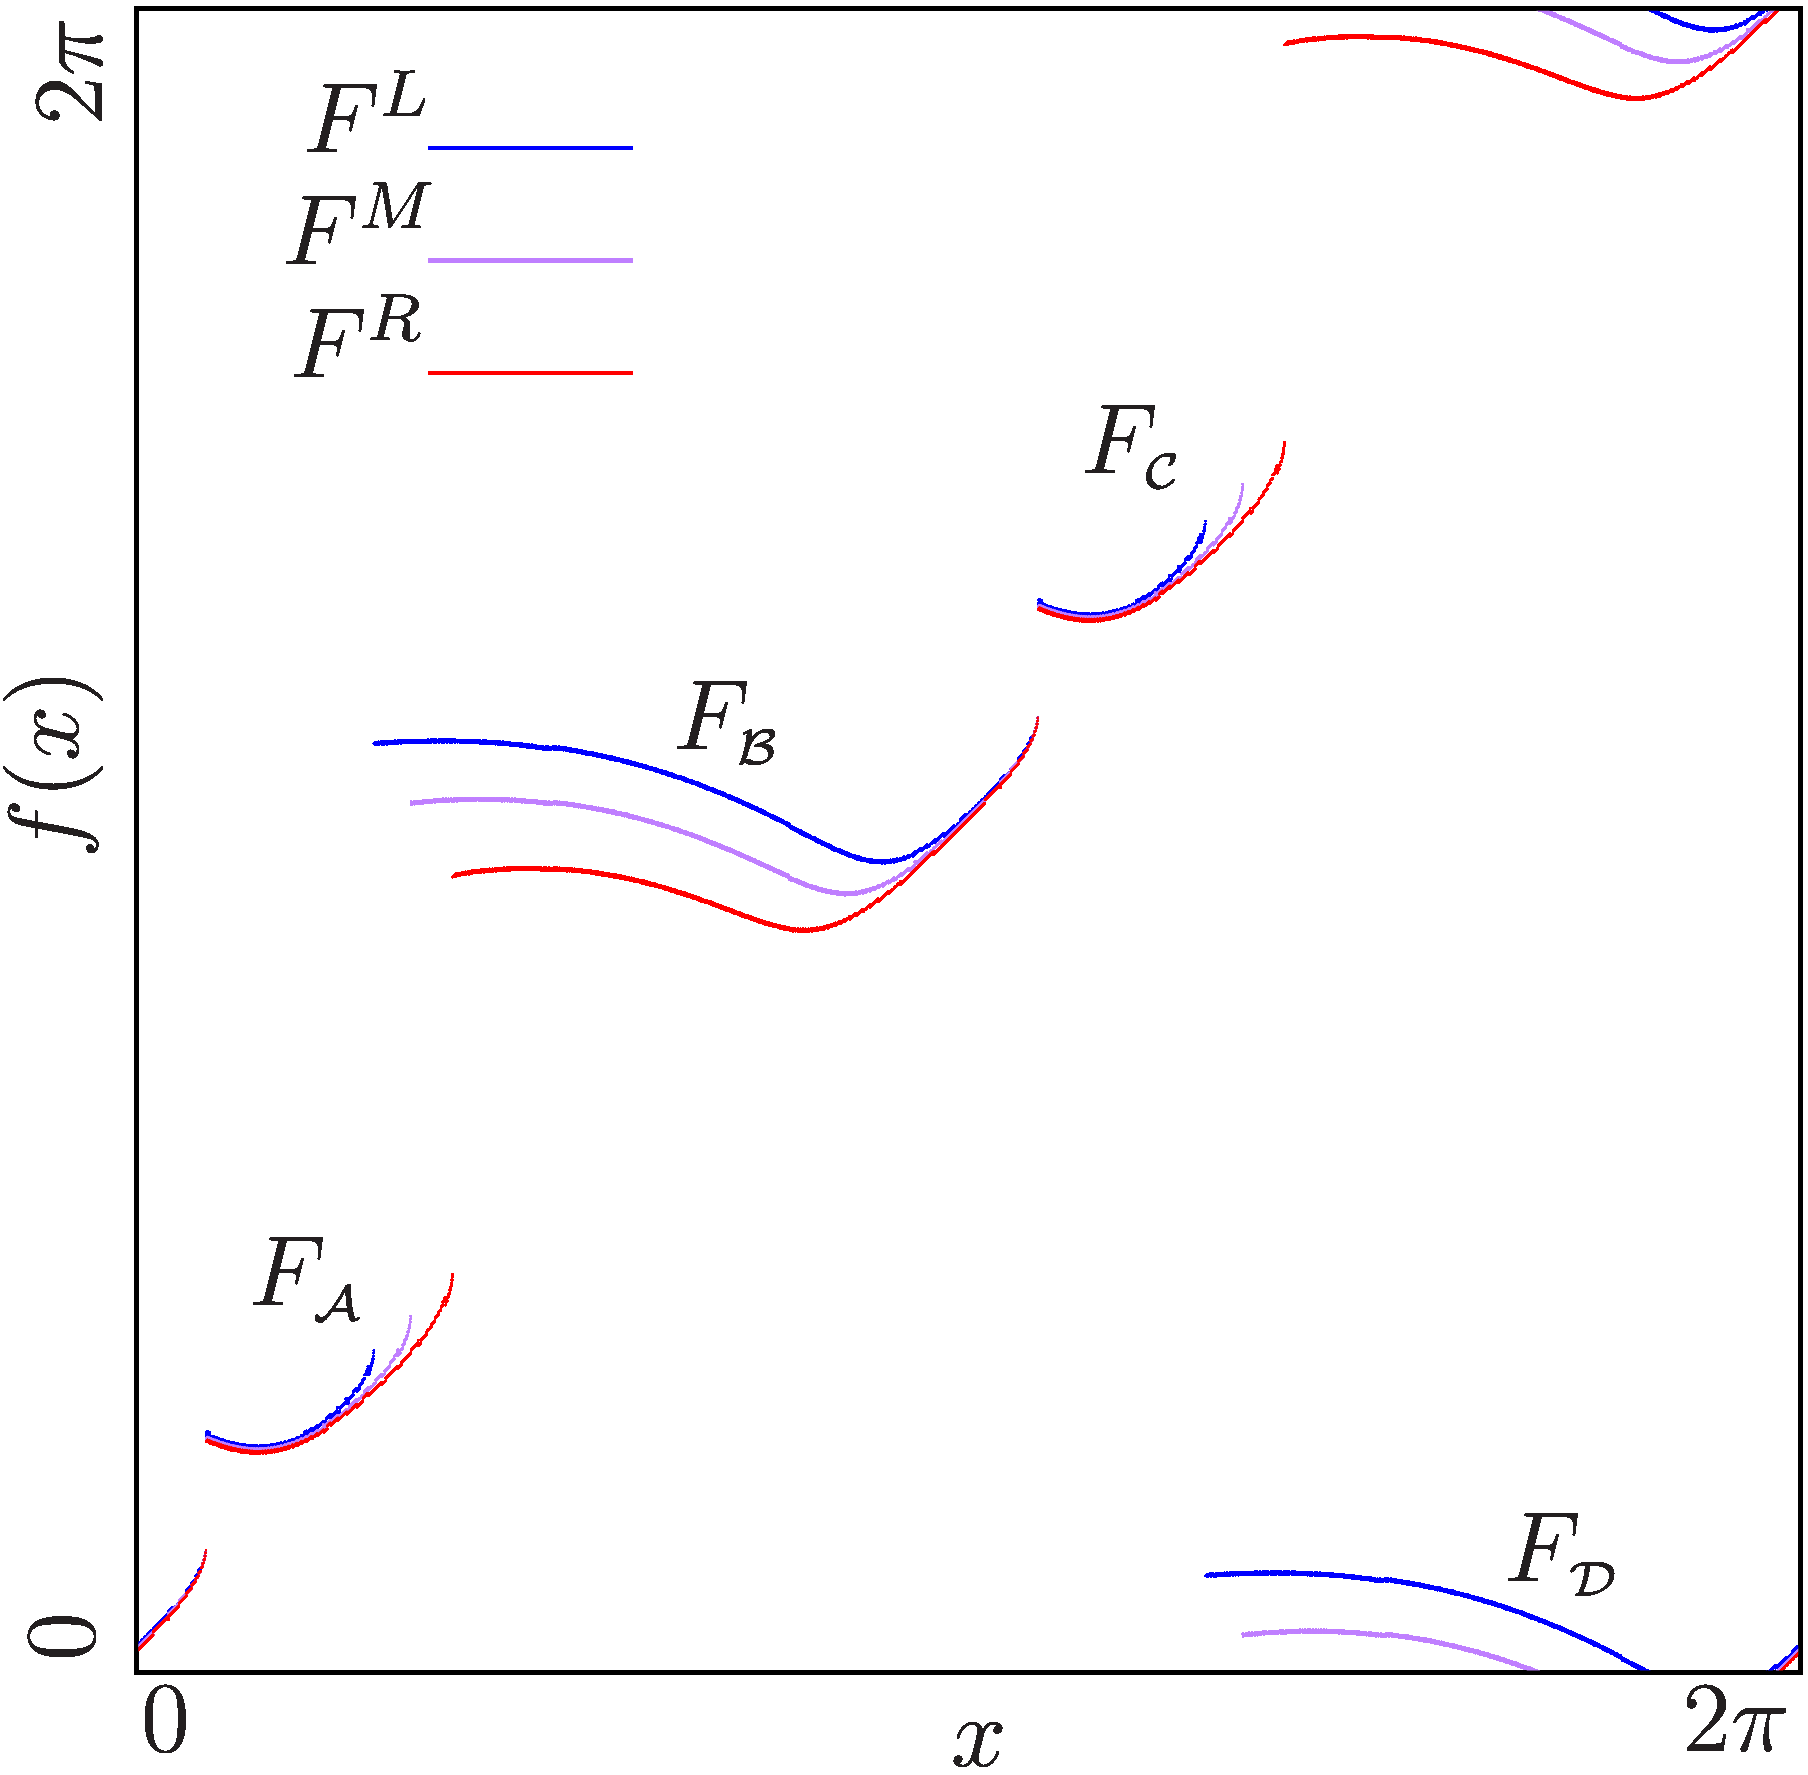
\includegraphics[width=0.2 \textwidth]{../Figures/5/5.4a/illustration.png}
		}{Effect of $E_0$}
		\stackunder[5pt]{
			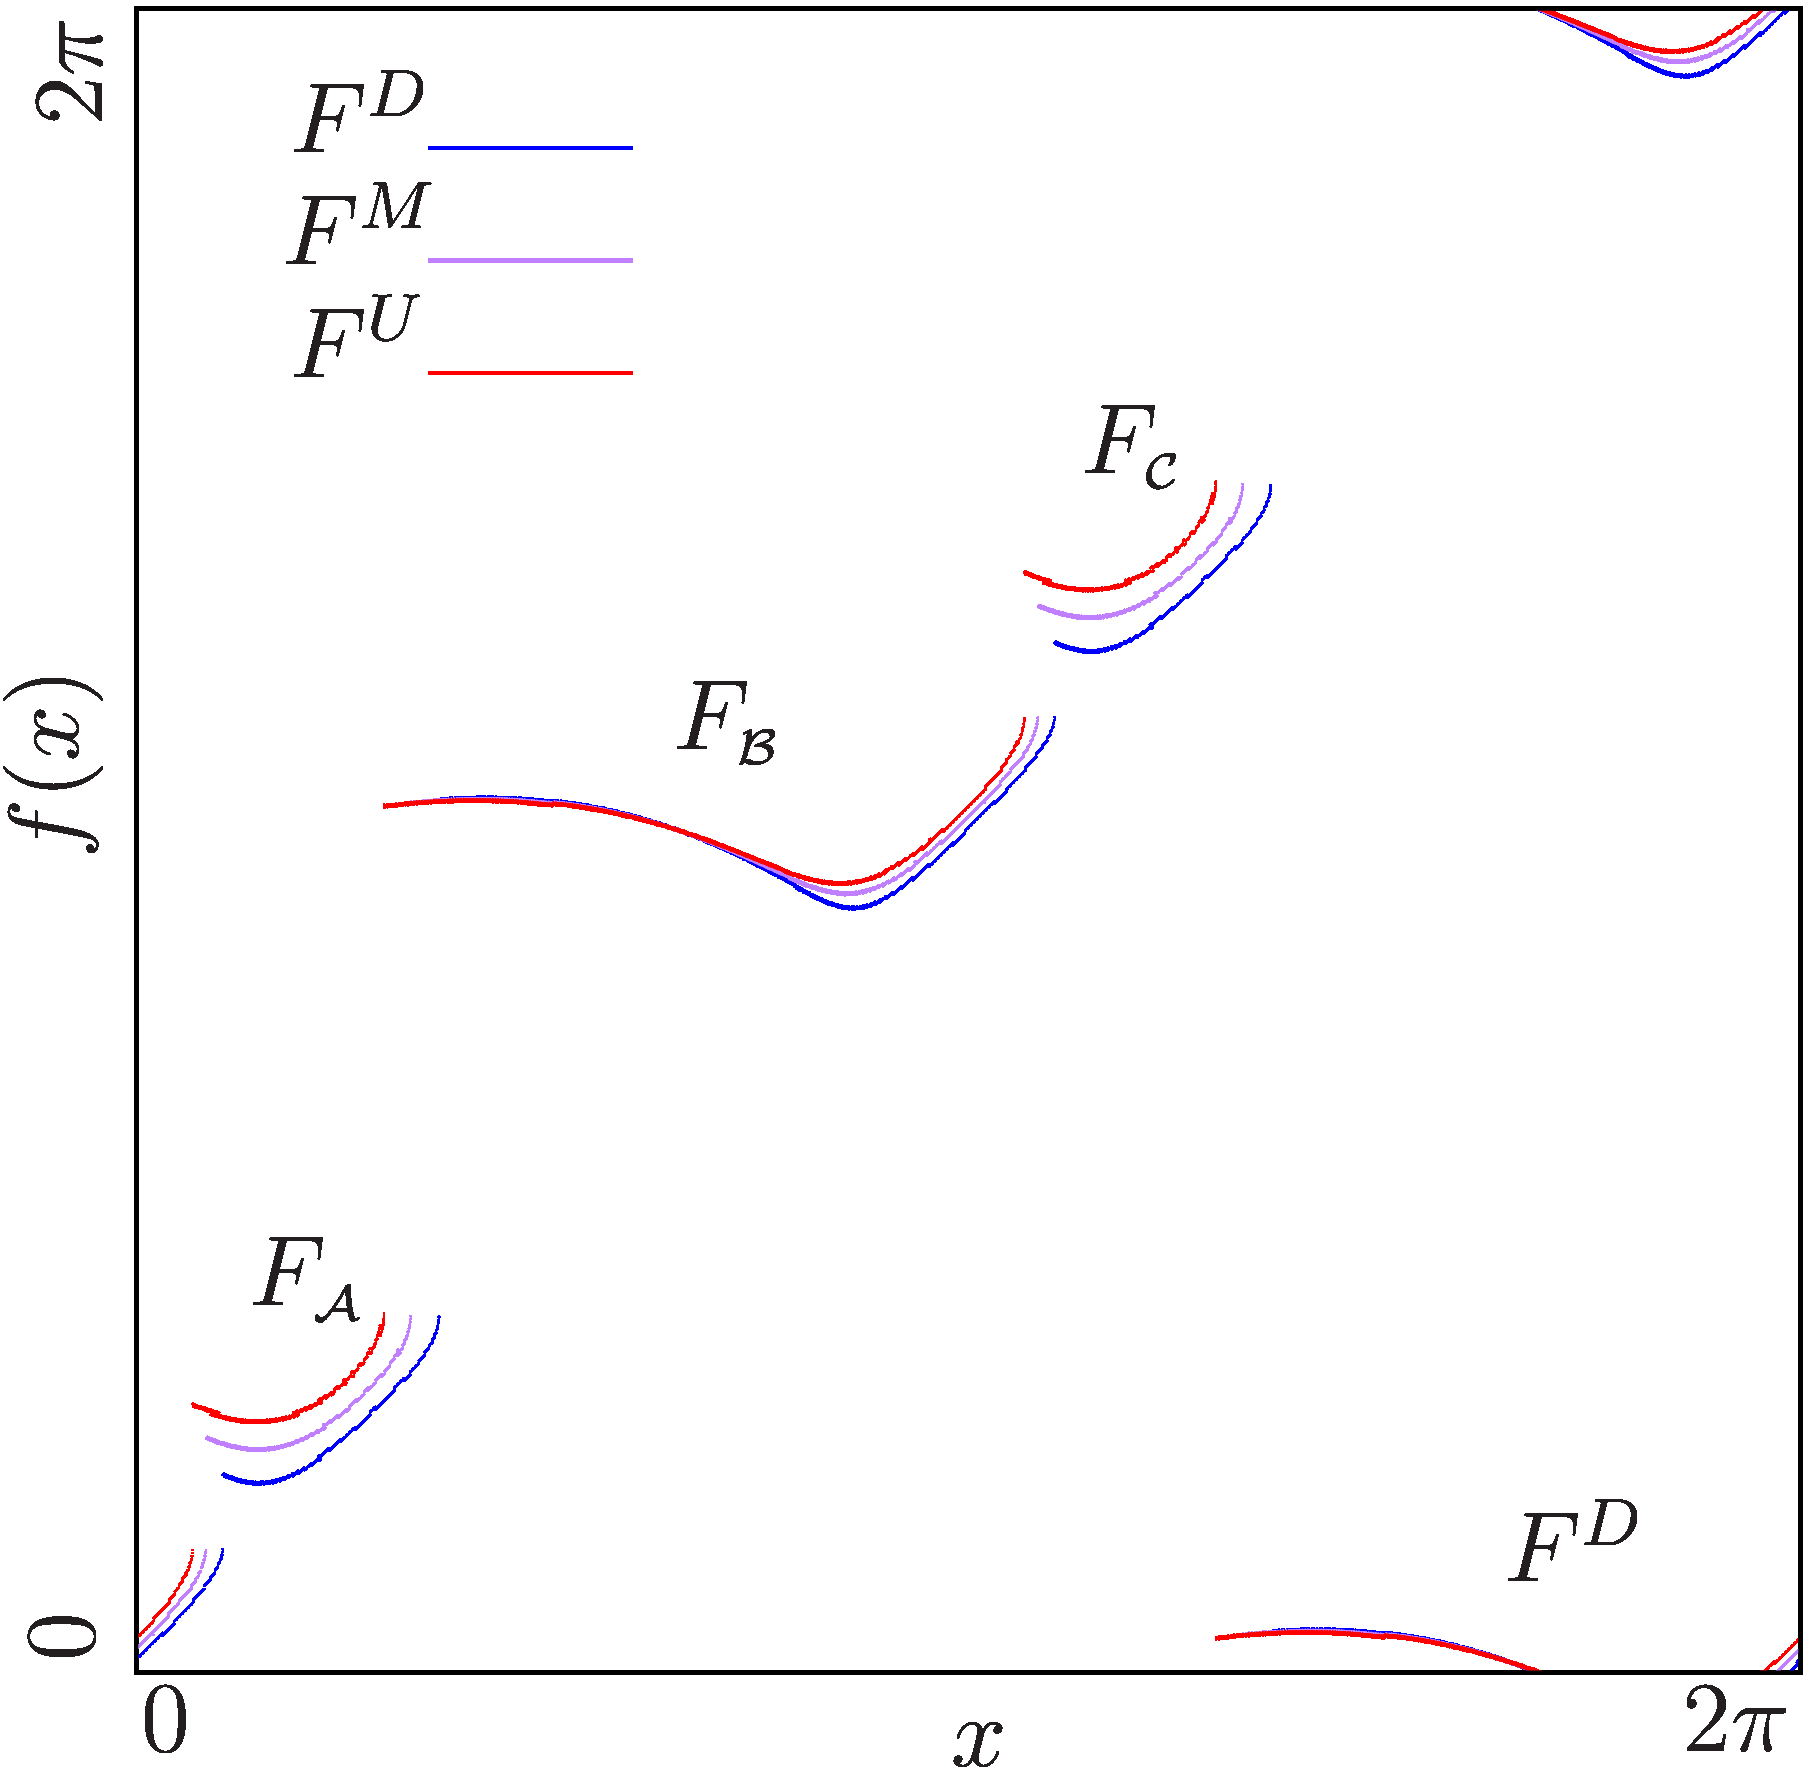
\includegraphics[width=0.2 \textwidth]{../Figures/5/5.4b/illustration.png}
		}{Effect of $\chi_0$}
		\stackunder[5pt]{
			\includegraphics[width=0.2 \textwidth]{60_MinimalRepr/ParameterEffects/p_x/illustration.png}
		}{Effect of $\alpha$}
		\stackunder[5pt]{
			\includegraphics[width=0.2 \textwidth]{60_MinimalRepr/ParameterEffects/p_y/illustration.png}
		}{Effect of $\beta$}
	\end{figure}
\end{frame}

\begin{frame}{Archetypal Model Dynamics}
	\only<1>{
		\vspace{-1em}
		\begin{figure}
			\stackunder[5pt]{
				\includegraphics[width=0.3 \textwidth]{99_Yunus/2D_Period_Zoomed/result.png}
			}{Original model}
			\qquad
			\stackunder[5pt]{
				\includegraphics[width=0.3 \textwidth]{60_MinimalRepr/2D_Period_Whole_noPoints/result.png}
			}{Archetypal model}
		\end{figure}
	}
	\only<2>{
		\begin{columns}
			\begin{column}{.9 \textwidth}
				\begin{figure}
					\centering
					\stackunder[5pt]{
						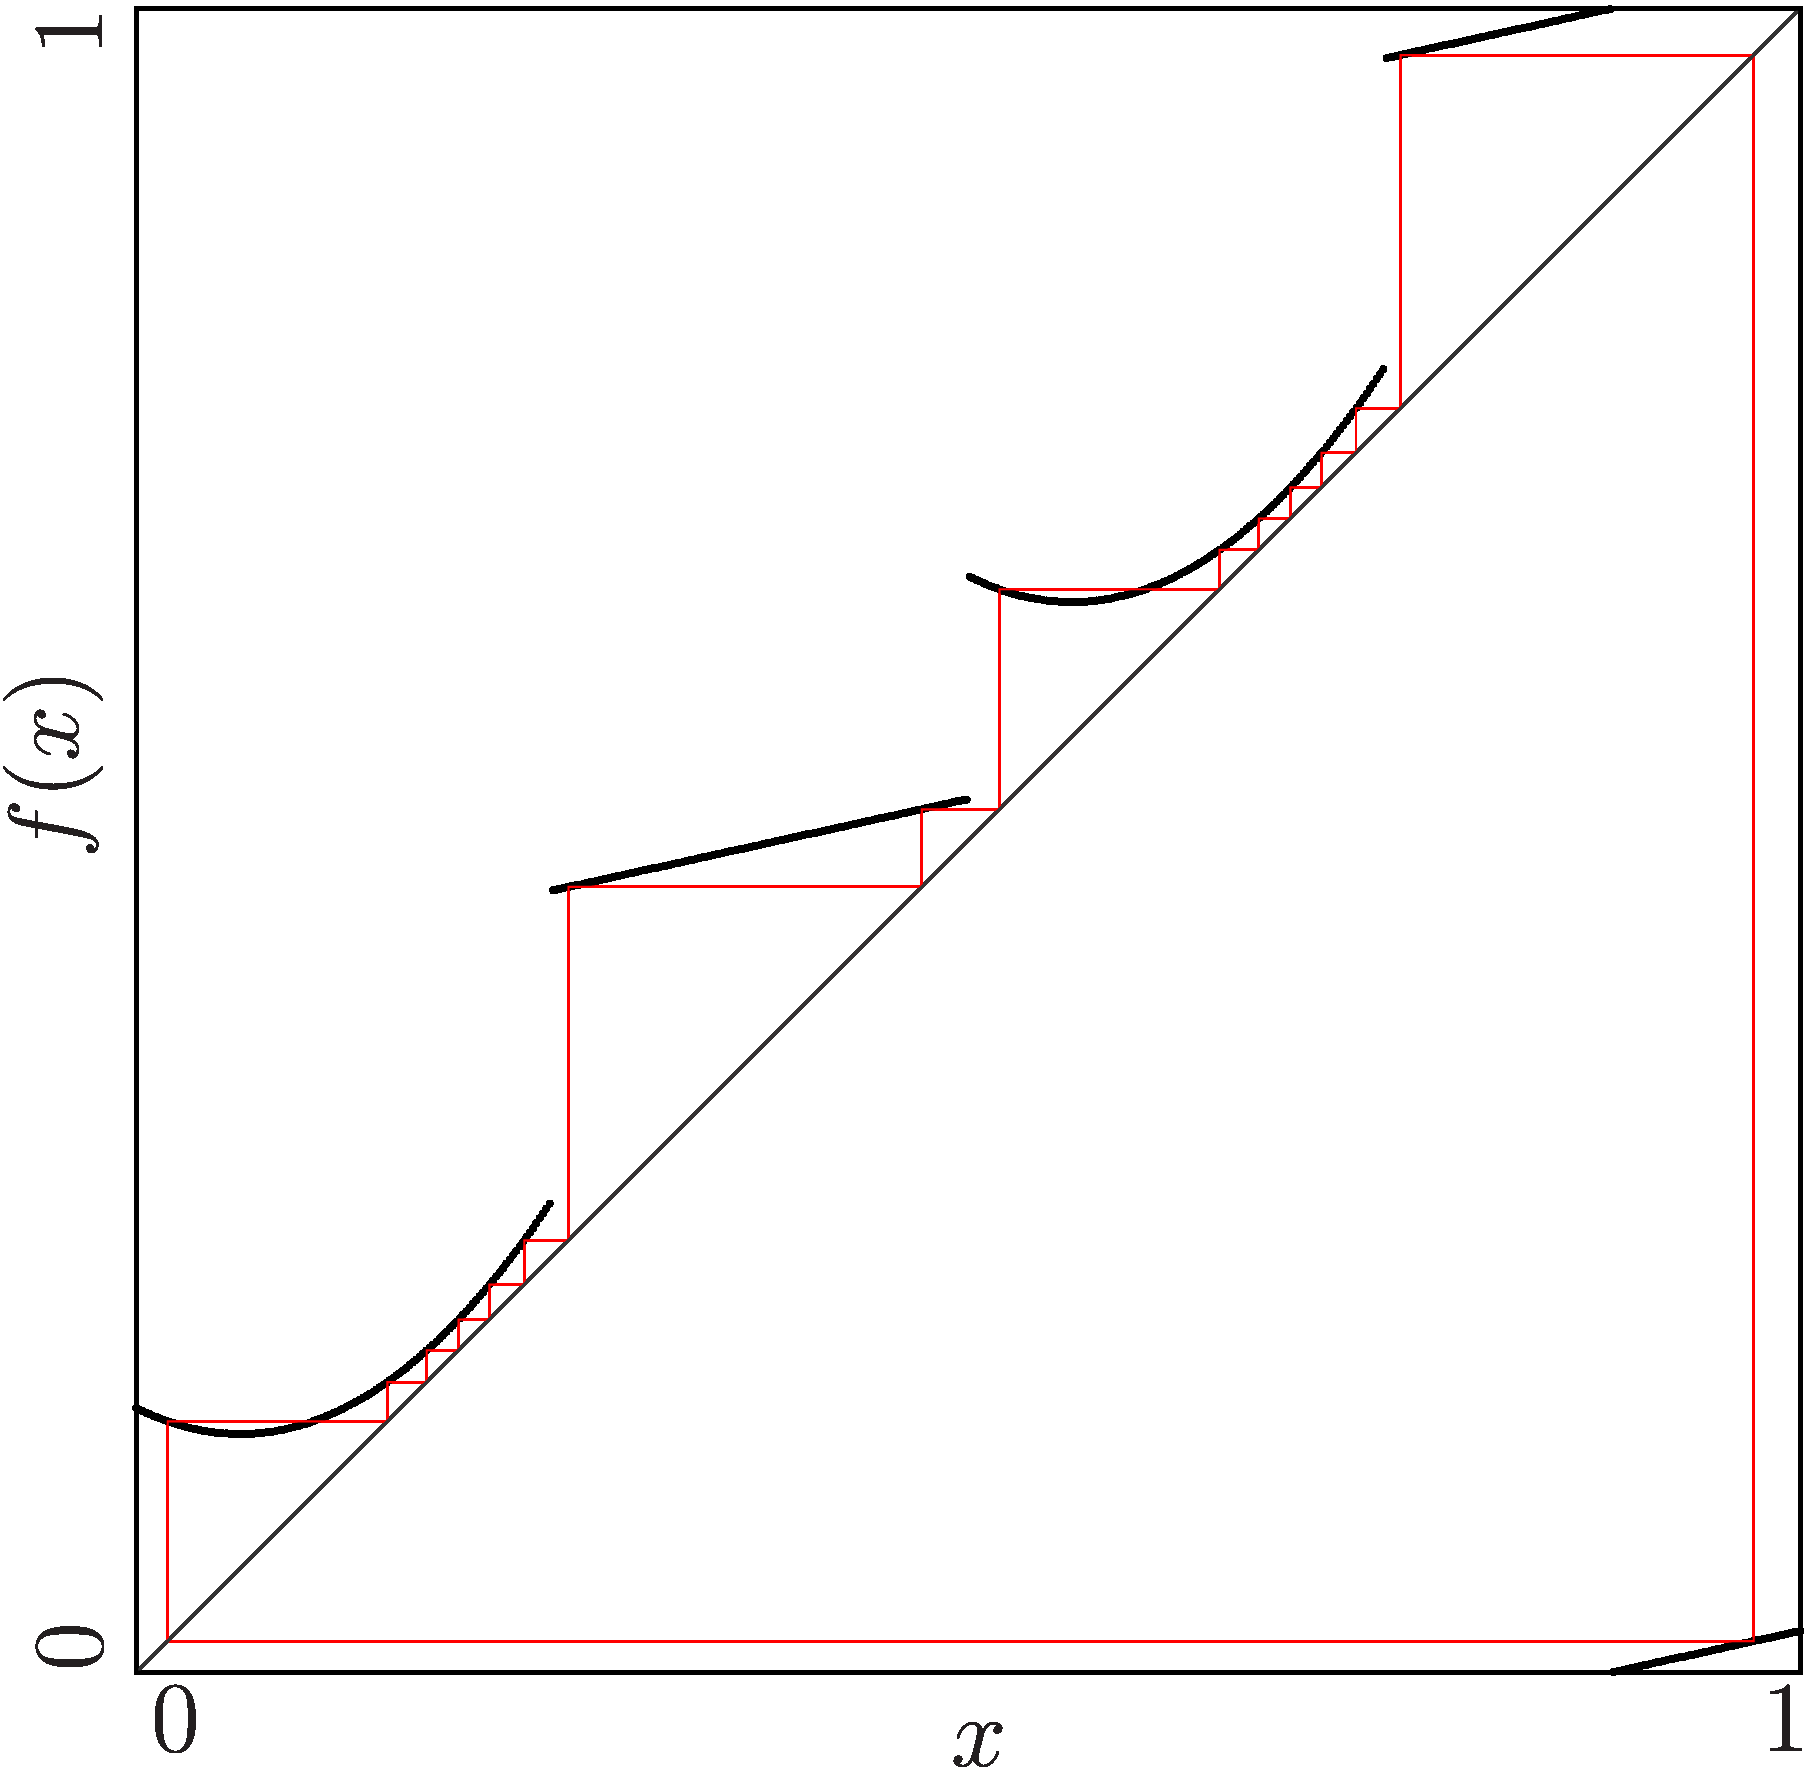
\includegraphics[height=0.45\textheight]{../Figures/6/6.2c/result.png}
					}{$C_{16}:\:\Cycle{\A^6\B^2\C^6\D^2}$}
					\stackunder[5pt]{
						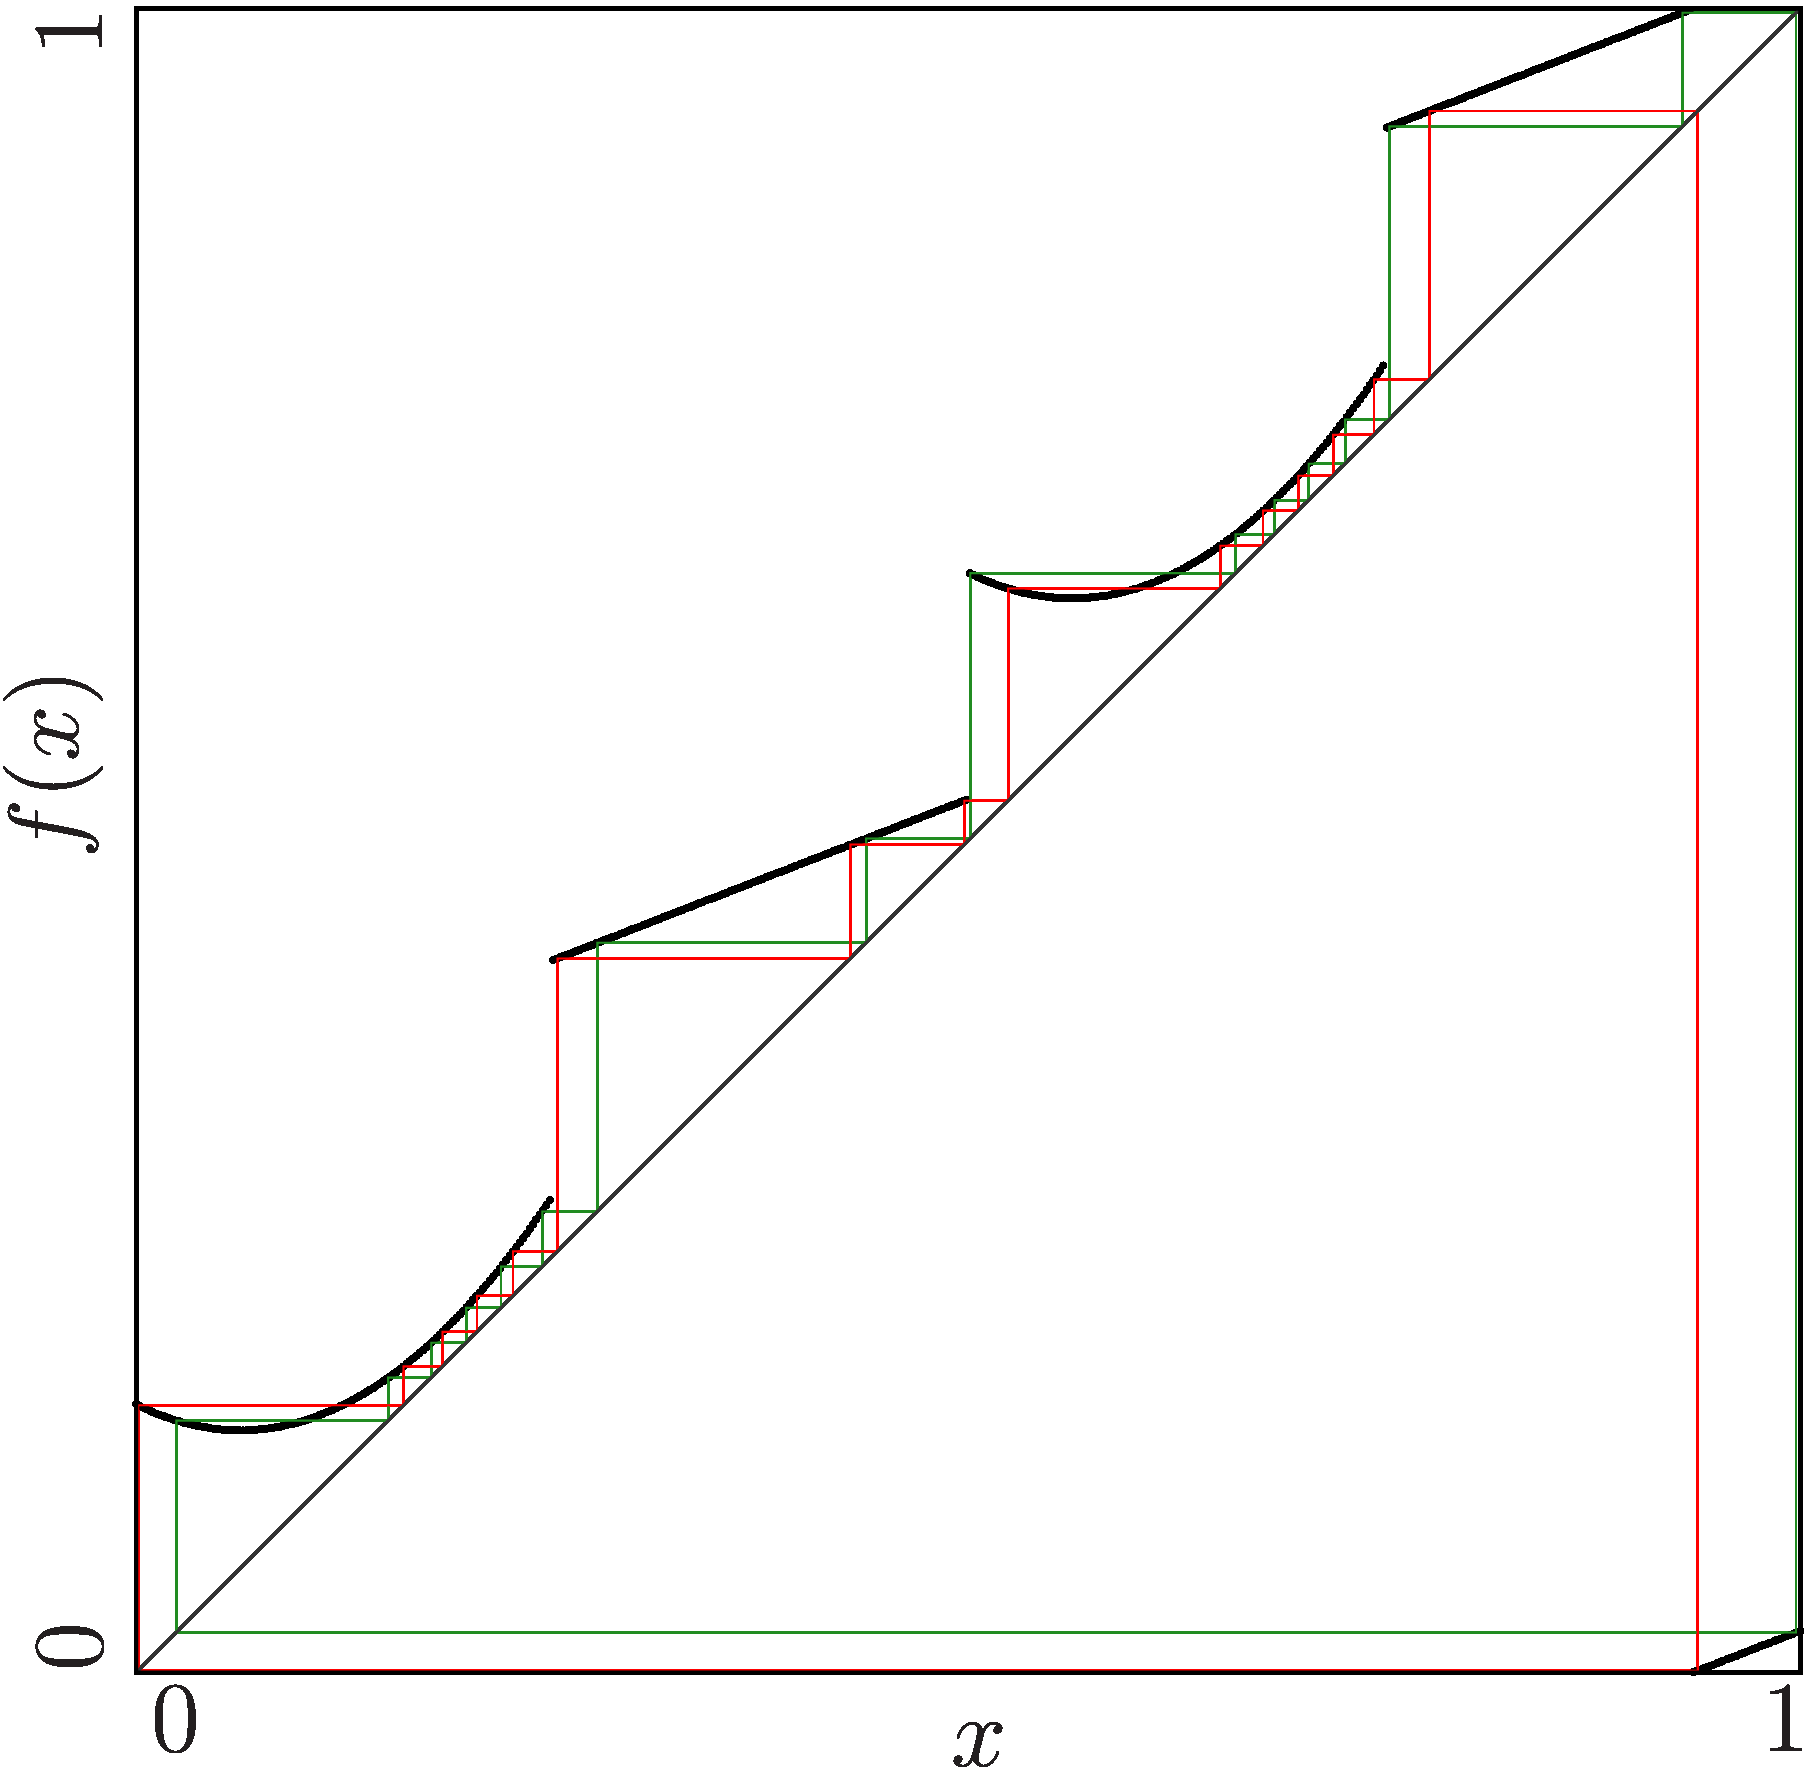
\includegraphics[height=0.45\textheight]{../Figures/6/6.2d/result.png}
					}{$D_{16}:\:\Cycle{\A^6\B^2\C^7\D^3},\Cycle{\A^7\B^3\C^6\D^2}$}
					\stackunder[5pt]{
						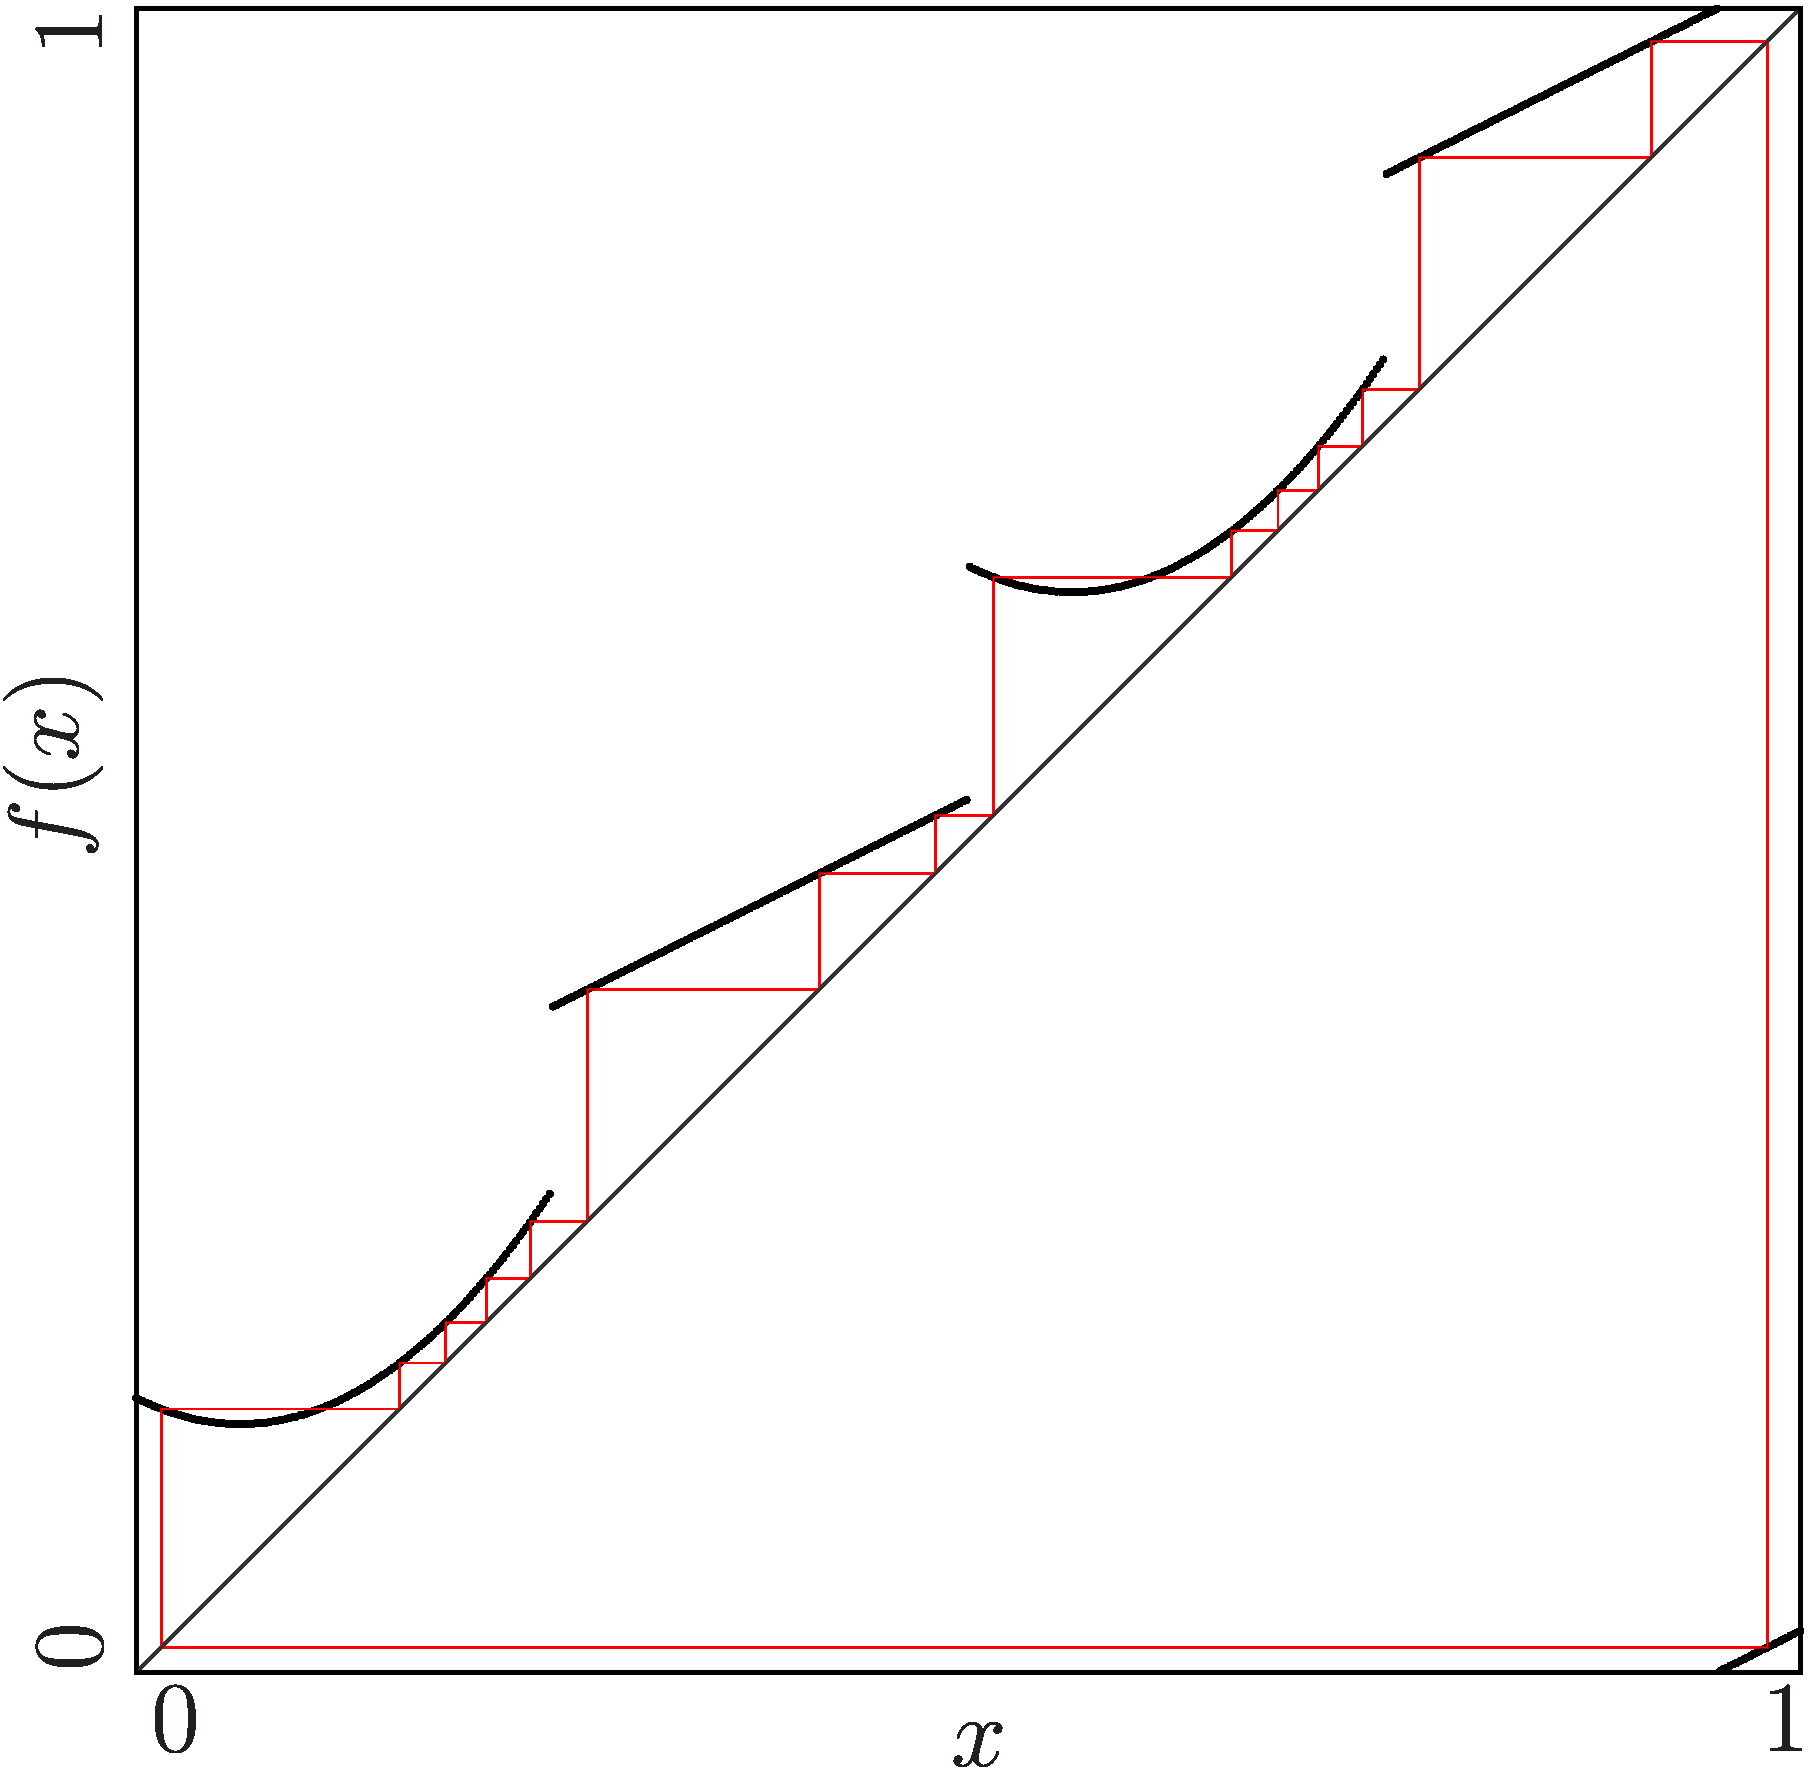
\includegraphics[height=0.45\textheight]{../Figures/6/6.2e/result.png}
					}{$E_{16}:\:\Cycle{\A^7\B^3\C^7\D^3}$}
				\end{figure}
			\end{column}
			\begin{column}{.2 \textwidth}
				\vspace{-4em}
				\begin{center}
					\hspace{-2em}
					\includegraphics[height=0.3 \textheight]{60_MinimalRepr/2D_Period_Whole_onlyP16_CDE/result.png}
				\end{center}
			\end{column}
		\end{columns}
	}
\end{frame}

\begin{frame}{Definition of the Archetypal Model (1/2)}
	\vspace{-3.0em}
	\begin{align}
		x_{n+1} = f(x_n) \mod 1
	\end{align}

	\begin{align}
		f(x) & = \begin{cases}
			         g(x)                                        & \text{ if } x < \frac{1}{2} \\
			         g\left(x - \frac{1}{2}\right) + \frac{1}{2} & \text{ else}
		         \end{cases}
	\end{align}

	\begin{align}
		g(x) & = \begin{cases}
			         g_L(x) = a_L \cdot x^2 + b_L \cdot x + c_L & \text{ if } x < \frac{1}{4} \\
			         g_R(x) = b_R \cdot x + c_R                 & \text{ else}
		         \end{cases}
	\end{align}
\end{frame}

\begin{frame}{Definition of the Archetypal Model (2/2)}
	\vspace{-1.5em}
	\begin{columns}
		\begin{column}{.7 \textwidth}
			Fixed parameters:
			\begin{align*}
				a_L = 4 \text{ and } b_L = -\frac{1}{2}
			\end{align*}
			Variable parameters
			\begin{align*}
				 & c_L, b_R, c_R                                                                                                           \\
				\text{where} \qquad
				 & c_L = \beta,                                                                                                            \\
				 & b_R = -4 \cdot g_R\left(\frac{1}{4}\right) + 4 \cdot g_R\left(\frac{1}{2}\right),                                       \\
				 & c_R = 2 \cdot g_R\left(\frac{1}{4}\right) - 1 \cdot g_R\left(\frac{1}{2}\right),                                        \\
				\text{and} \qquad
				 & g_R\left(\frac{1}{4}\right) = \alpha, \text{and } g_R\left(\frac{1}{2}\right) = \frac{1}{2} + \epsilon \text{ is fixed}
			\end{align*}
		\end{column}
		\begin{column}{.3 \textwidth}
			\begin{figure}
				\centering
				\includegraphics[height=.5 \textheight]{60_MinimalRepr/ParameterEffects/AB/illustration.png}
				%\caption*{Illustration of the parameters $A$ and $B$}
			\end{figure}
		\end{column}
	\end{columns}
\end{frame}

%\begin{frame}{Symbolic Sequences}
%	Cycles are described using symbolic sequences.
%	Symbols indicate which branches the points of the cycle are on.
%	\vspace{.5em}
%	\begin{columns}
%		\hspace{5em}
%		\begin{column}{.3 \textwidth}
%			\begin{figure}
%				\includegraphics[width=\textwidth]{60_MinimalRepr/Cobweb_E16/result.png}
%			\end{figure}
%		\end{column}
%		\hspace{3em}
%		\begin{column}{.6 \textwidth}
%			\begin{itemize}
%				\item Cycle of period 16
%				\item Symbolic Sequence: $\A^5\B^3\C^5\D^3$
%			\end{itemize}
%		\end{column}
%	\end{columns}
%\end{frame}

%\begin{frame}{Parameter Regions in Minimal Reproducing Model}
%	\begin{itemize}
%		\item ``Type A'': At points $C_{16}$ and $E_{16}$ in 2D scan
%		      \begin{itemize}
%			      \item One cycle
%			      \item Symmetrical
%			      \item Example at point $C_{16}$: $\Cycle{\A^6\B^2\C^6\D^2}$
%			      \item Example at point $E_{16}$: $\Cycle{\A^5\B^3\C^5\D^3}$ \vspace*{1em}
%		      \end{itemize}
%		\item ``Type B'': At point $D_{16}$ in 2D scan
%		      \begin{itemize}
%			      \item Two coexisting cycles
%			      \item Asymmetrical
%			      \item Example at point $D_{16}$: $\Cycle{\A^6\B^2\C^5\D^3}$ and $\Cycle{\A^5\B^3\C^6\D^2}$
%		      \end{itemize}
%	\end{itemize}
%\end{frame}


\begin{frame}{Bifurcation Analysis}
	\vspace{-1em}
	\begin{columns}
		\begin{column}{.5 \textwidth}
			At the boundaries of the ``type B'' period region with the cycles $\Cycle{\A^5\B^3\C^4\D^4}$ and $\Cycle{\A^4\B^4\C^5\D^3}$
			\pause
			\begin{itemize}
				\item Always border collision bifurcations
				\item Unusual \begin{itemize}
					      \item ``Type B'' coexisting cycles collide with two borders at the same bifurcation
					      \item ``Type A'' cycles collide with two borders at the same bifurcation
				      \end{itemize}
			\end{itemize}
			\vspace{.5em}
			The borders, the cycles collide with at the same bifurcation are at $x$ and $(x + \frac{1}{2}) \mod 1$ (due to the symmetry)
		\end{column}
		\begin{column}{.5 \textwidth}
			\vspace{-5em}
			\begin{figure}
				\centering
				\only<1>{
					\vspace{3em}
					\subfloat{ 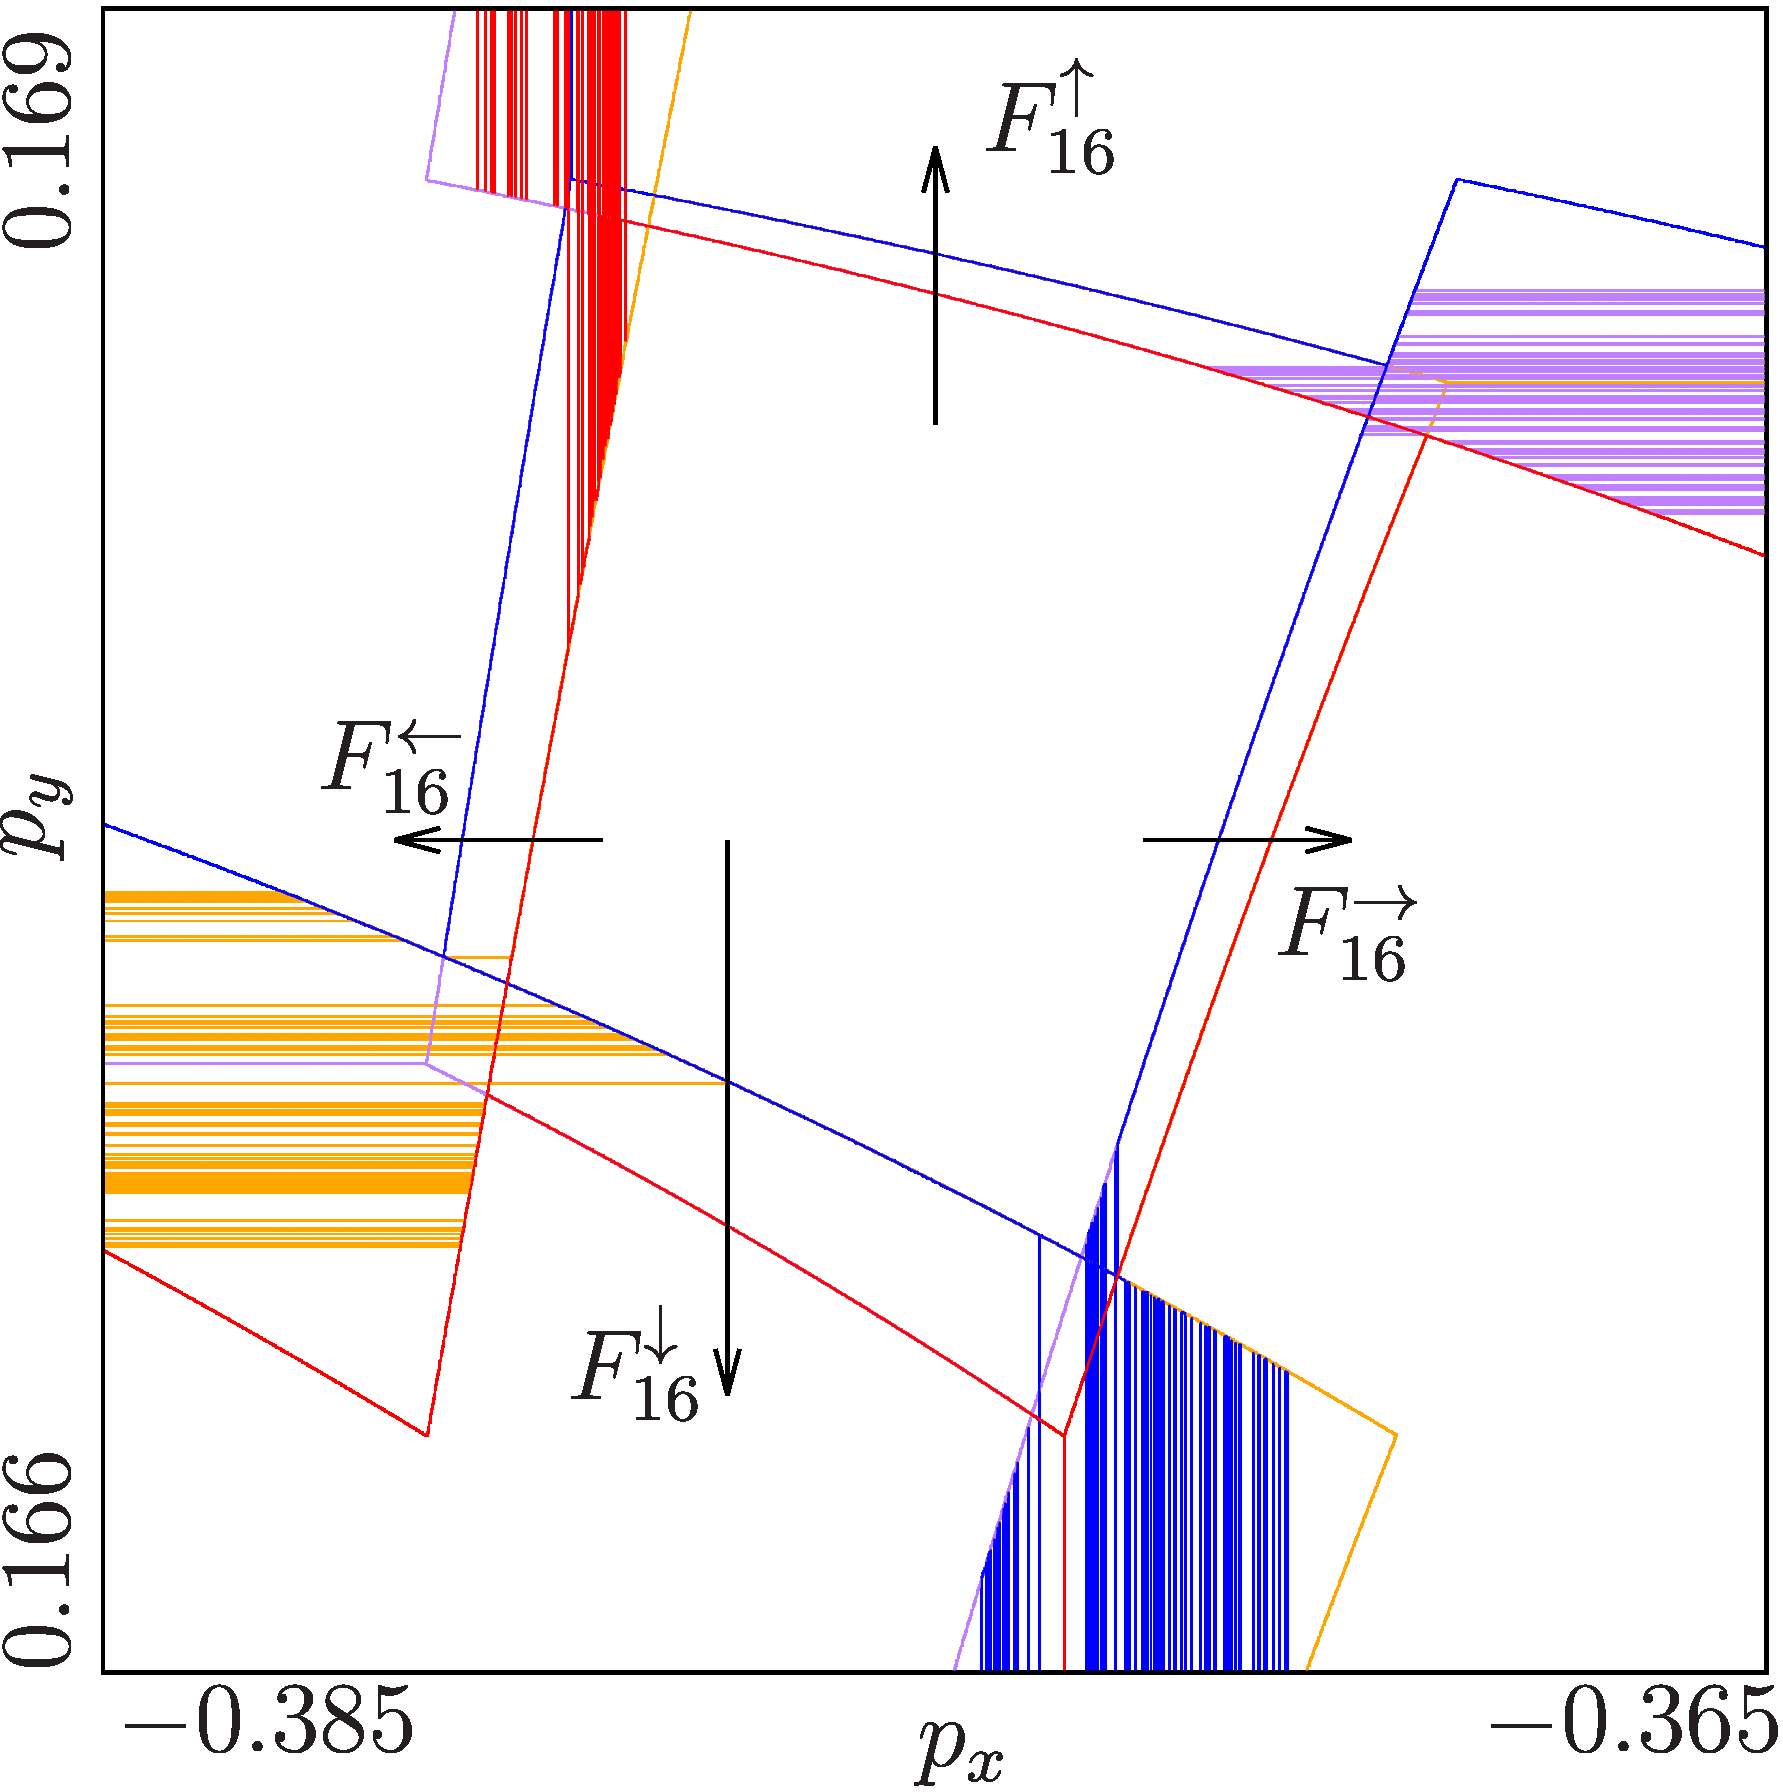
\includegraphics[height=.7 \textheight]{../Figures/6/6.3b/result.png} }
				}
				\only<2->{
					\subfloat{ 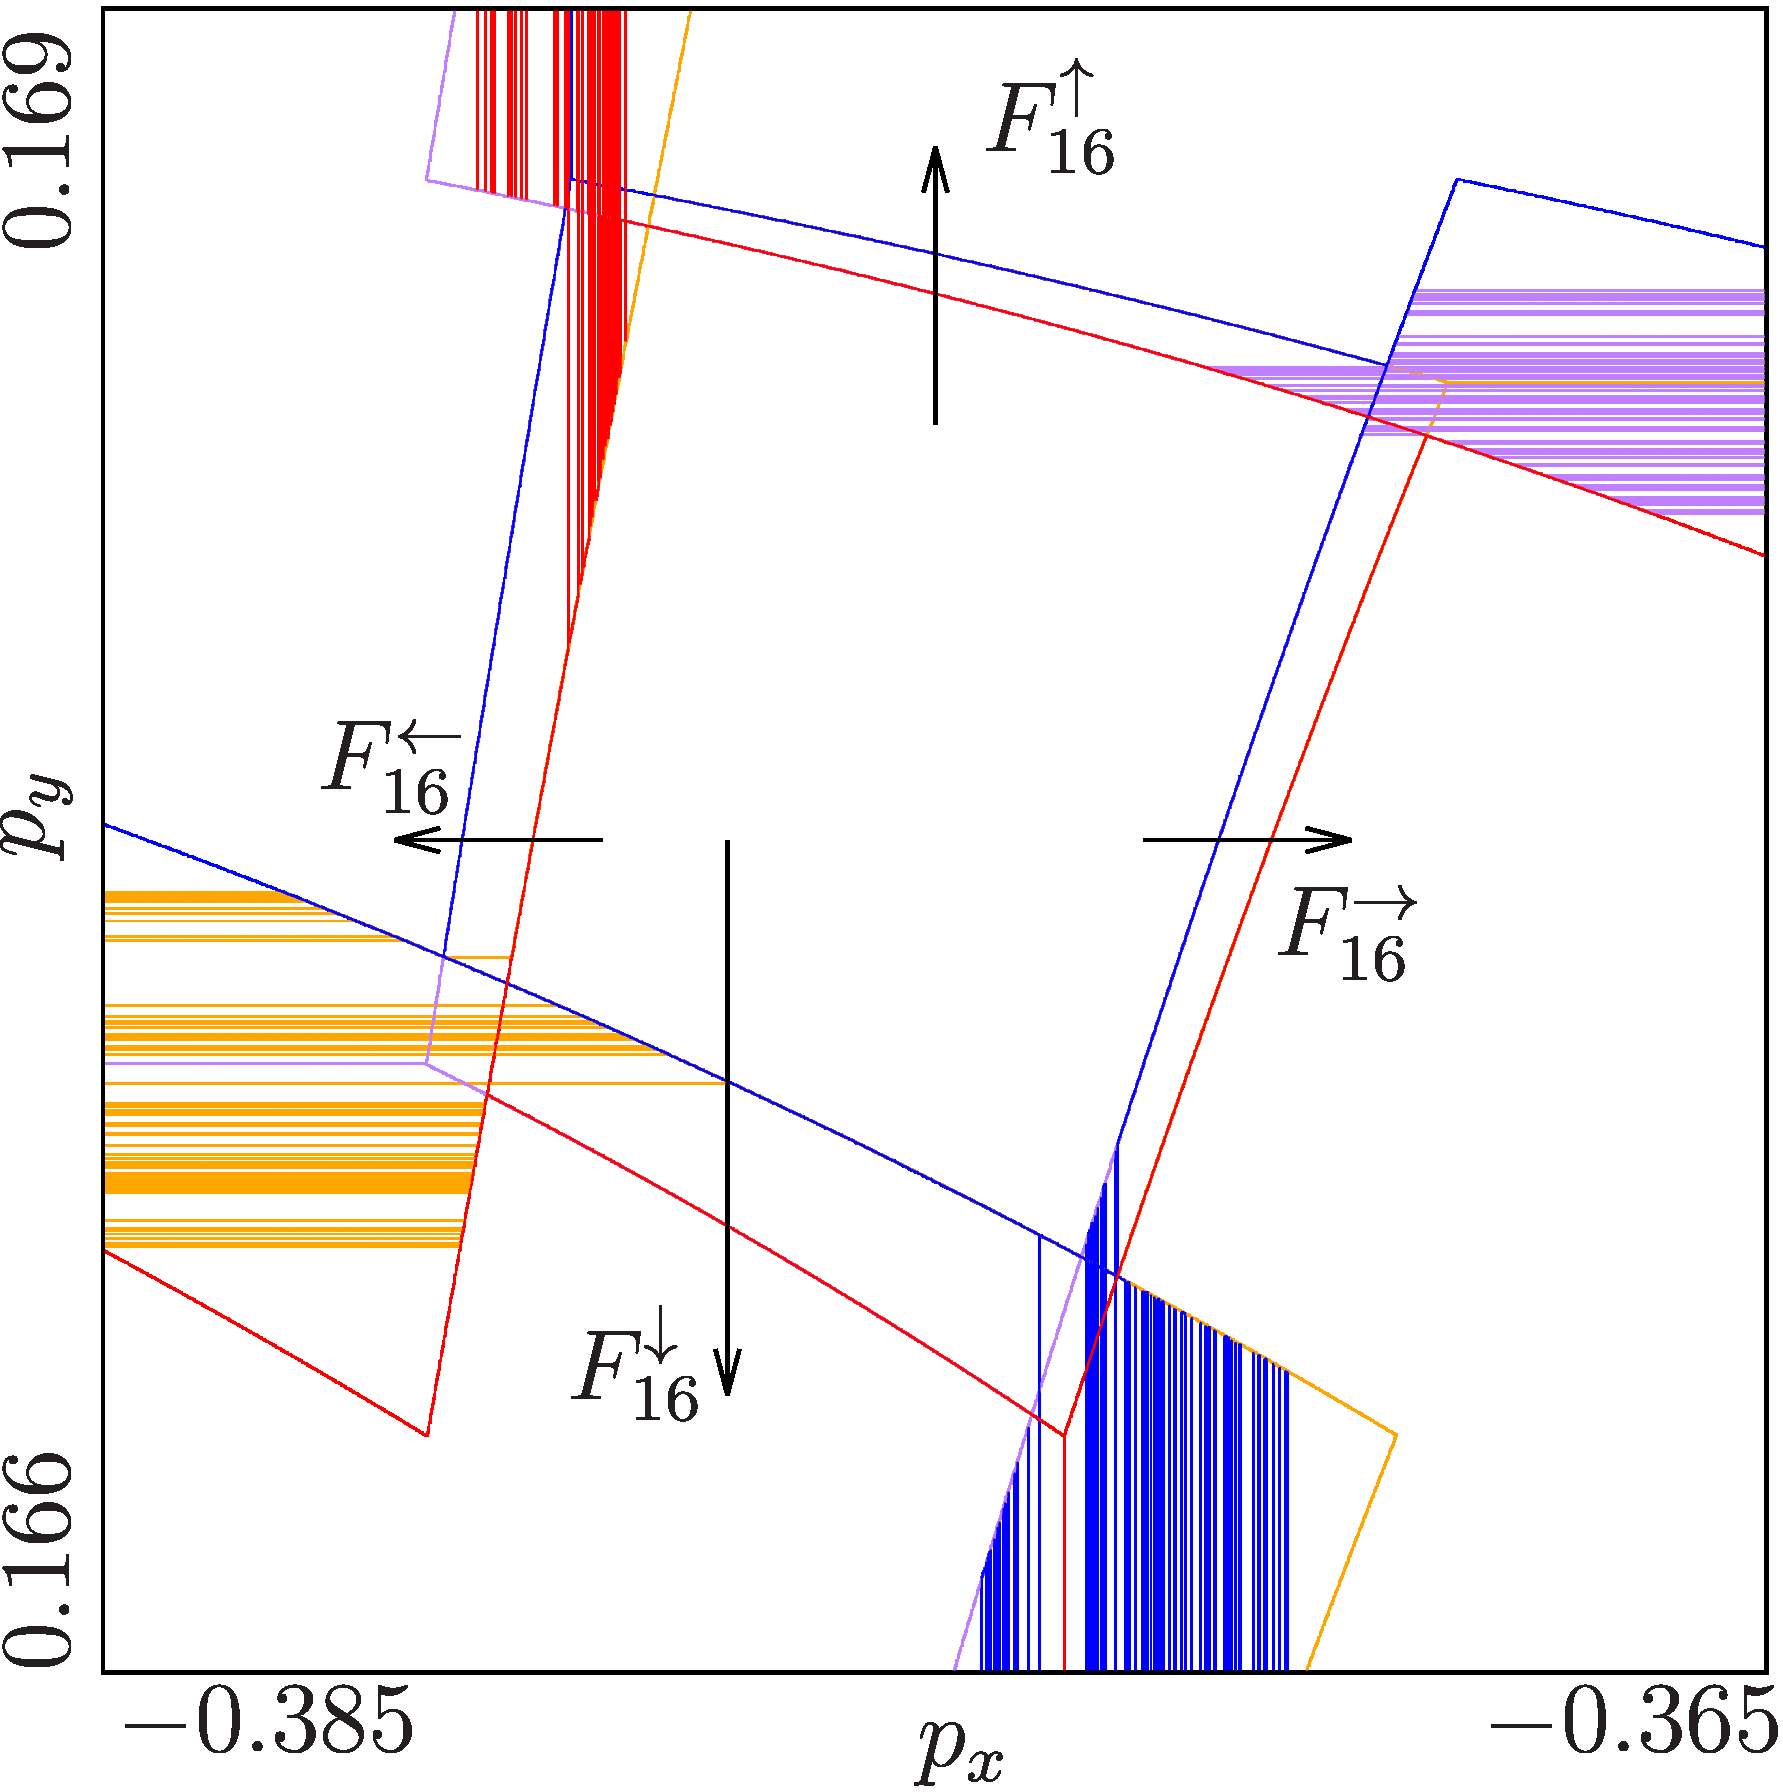
\includegraphics[height=.2 \textheight]{../Figures/6/6.3b/result.png} }
				}
				\only<2>{
					\subfloat{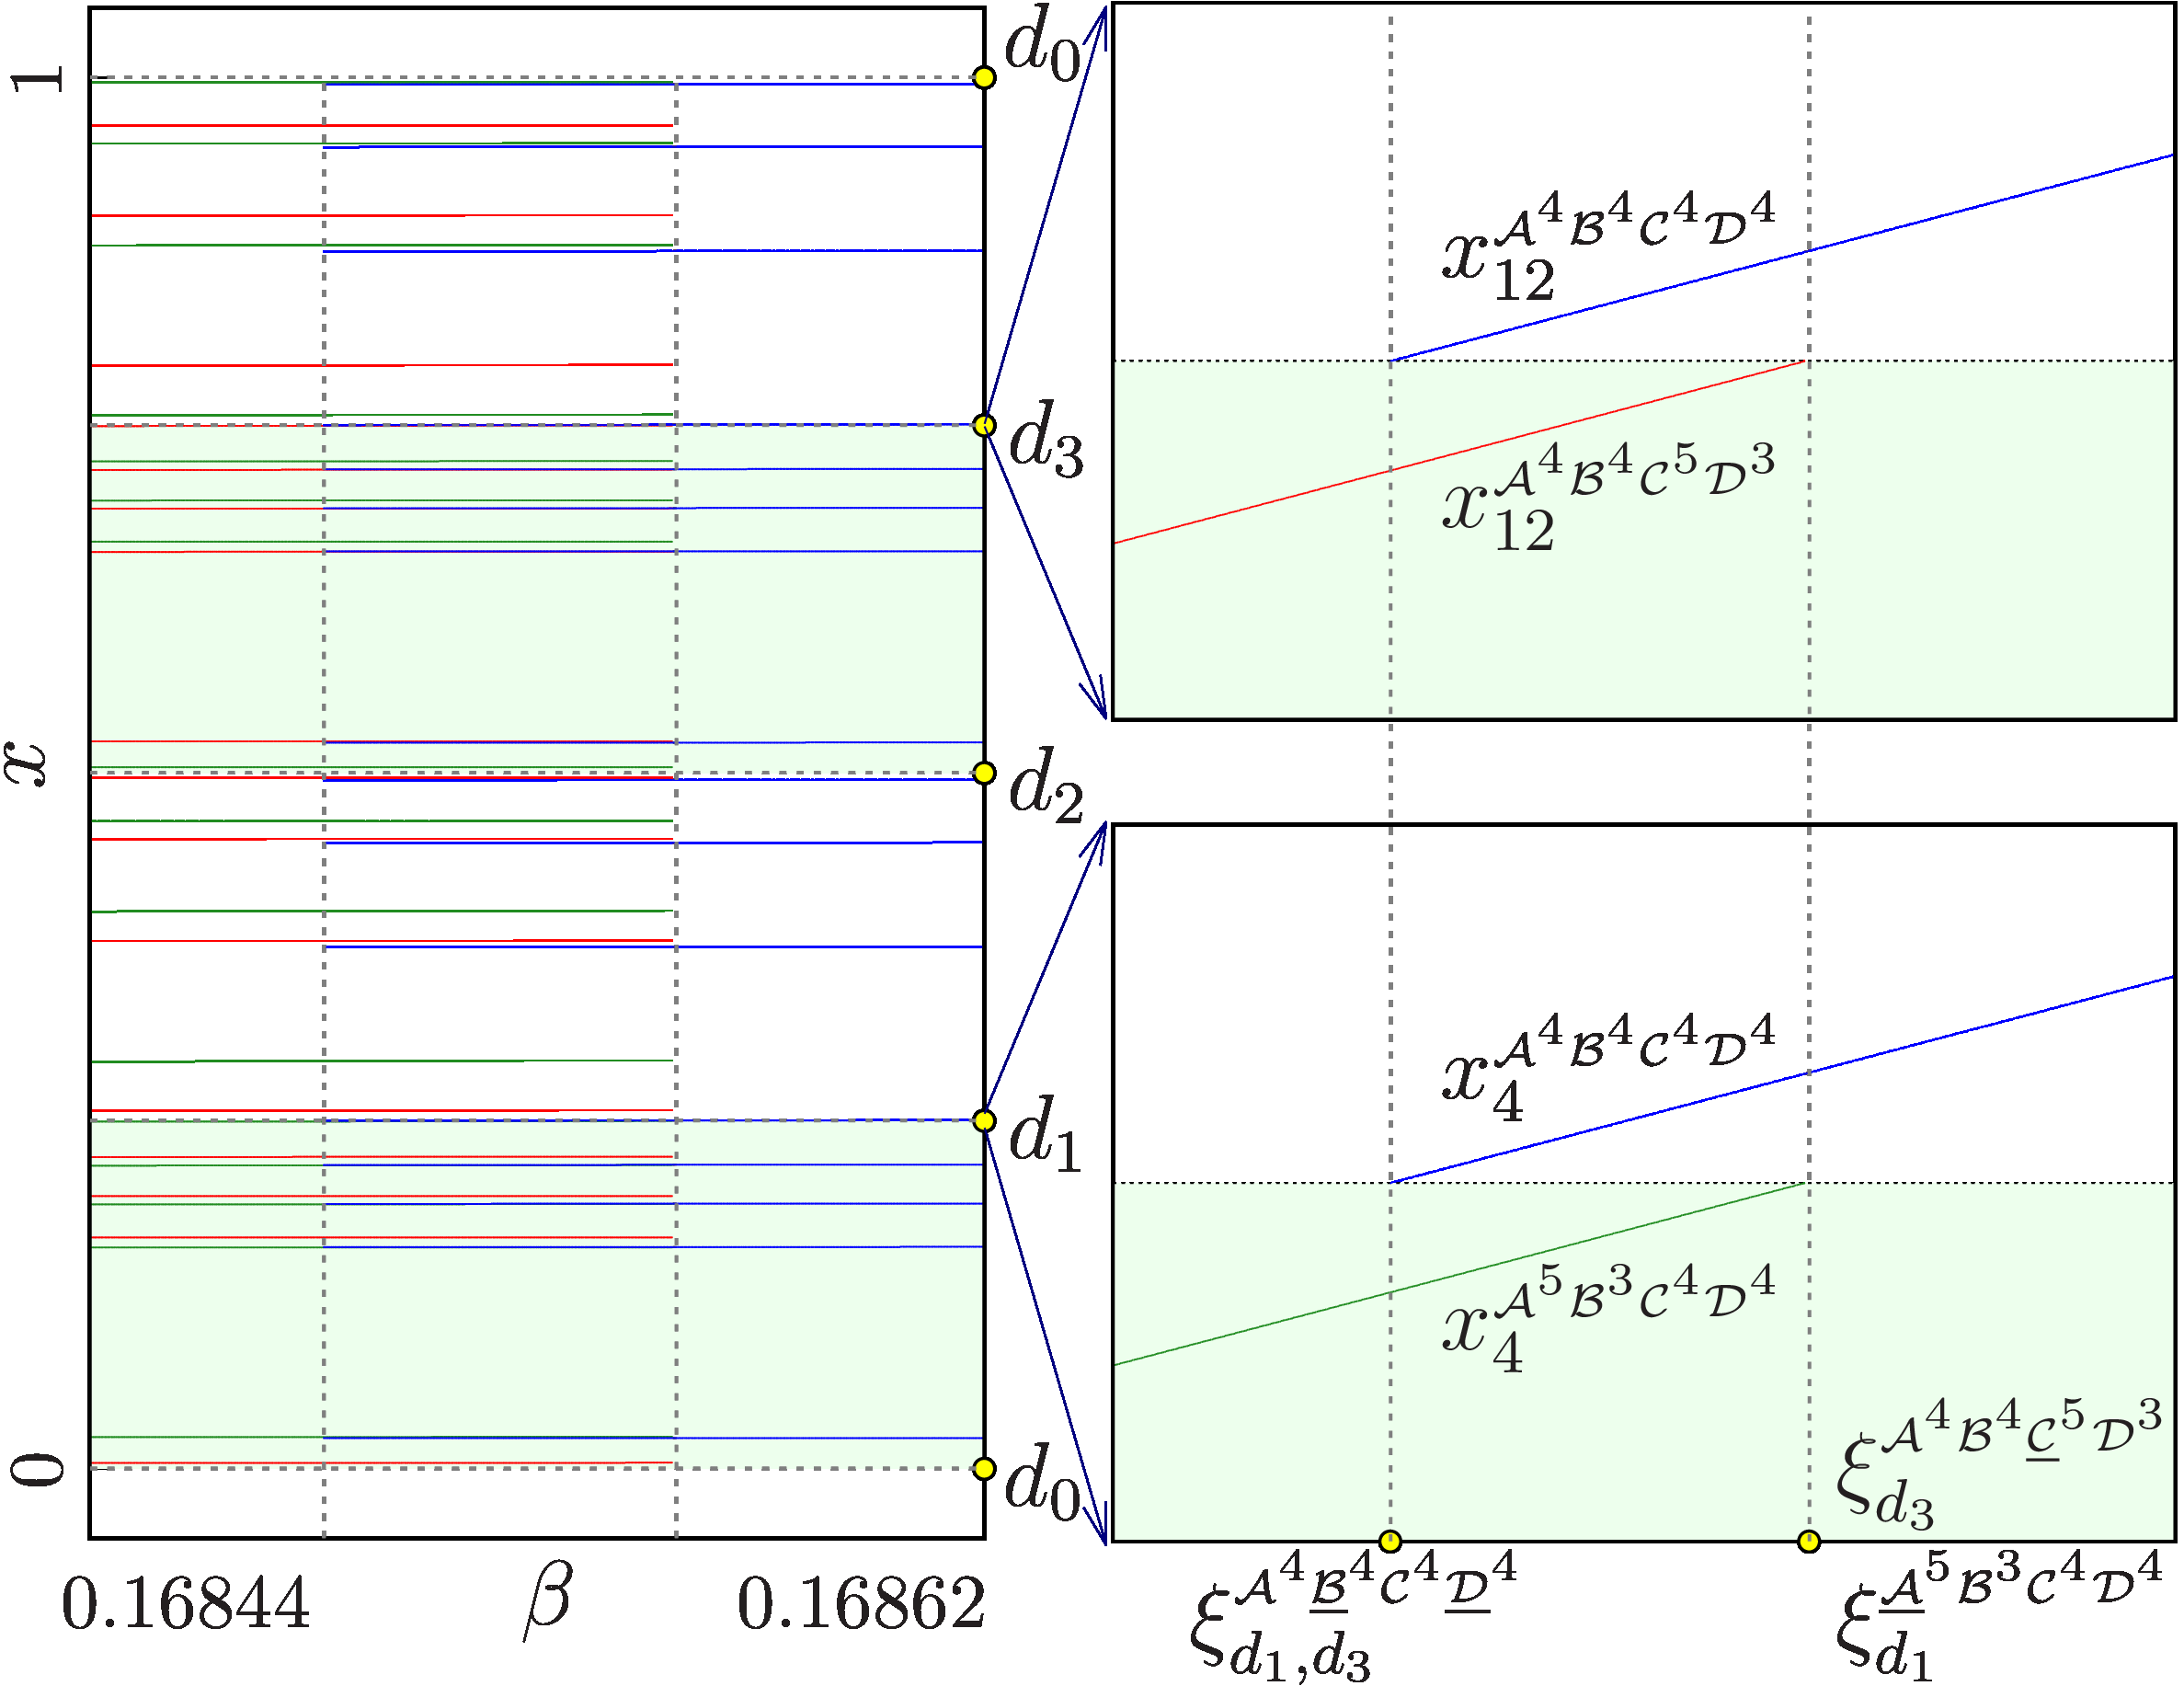
\includegraphics[height=.7 \textheight]{../Figures/6/6.4/result.png}}
					\caption*{$F_{16}^\uparrow$}
				}
				\only<3>{
					\subfloat{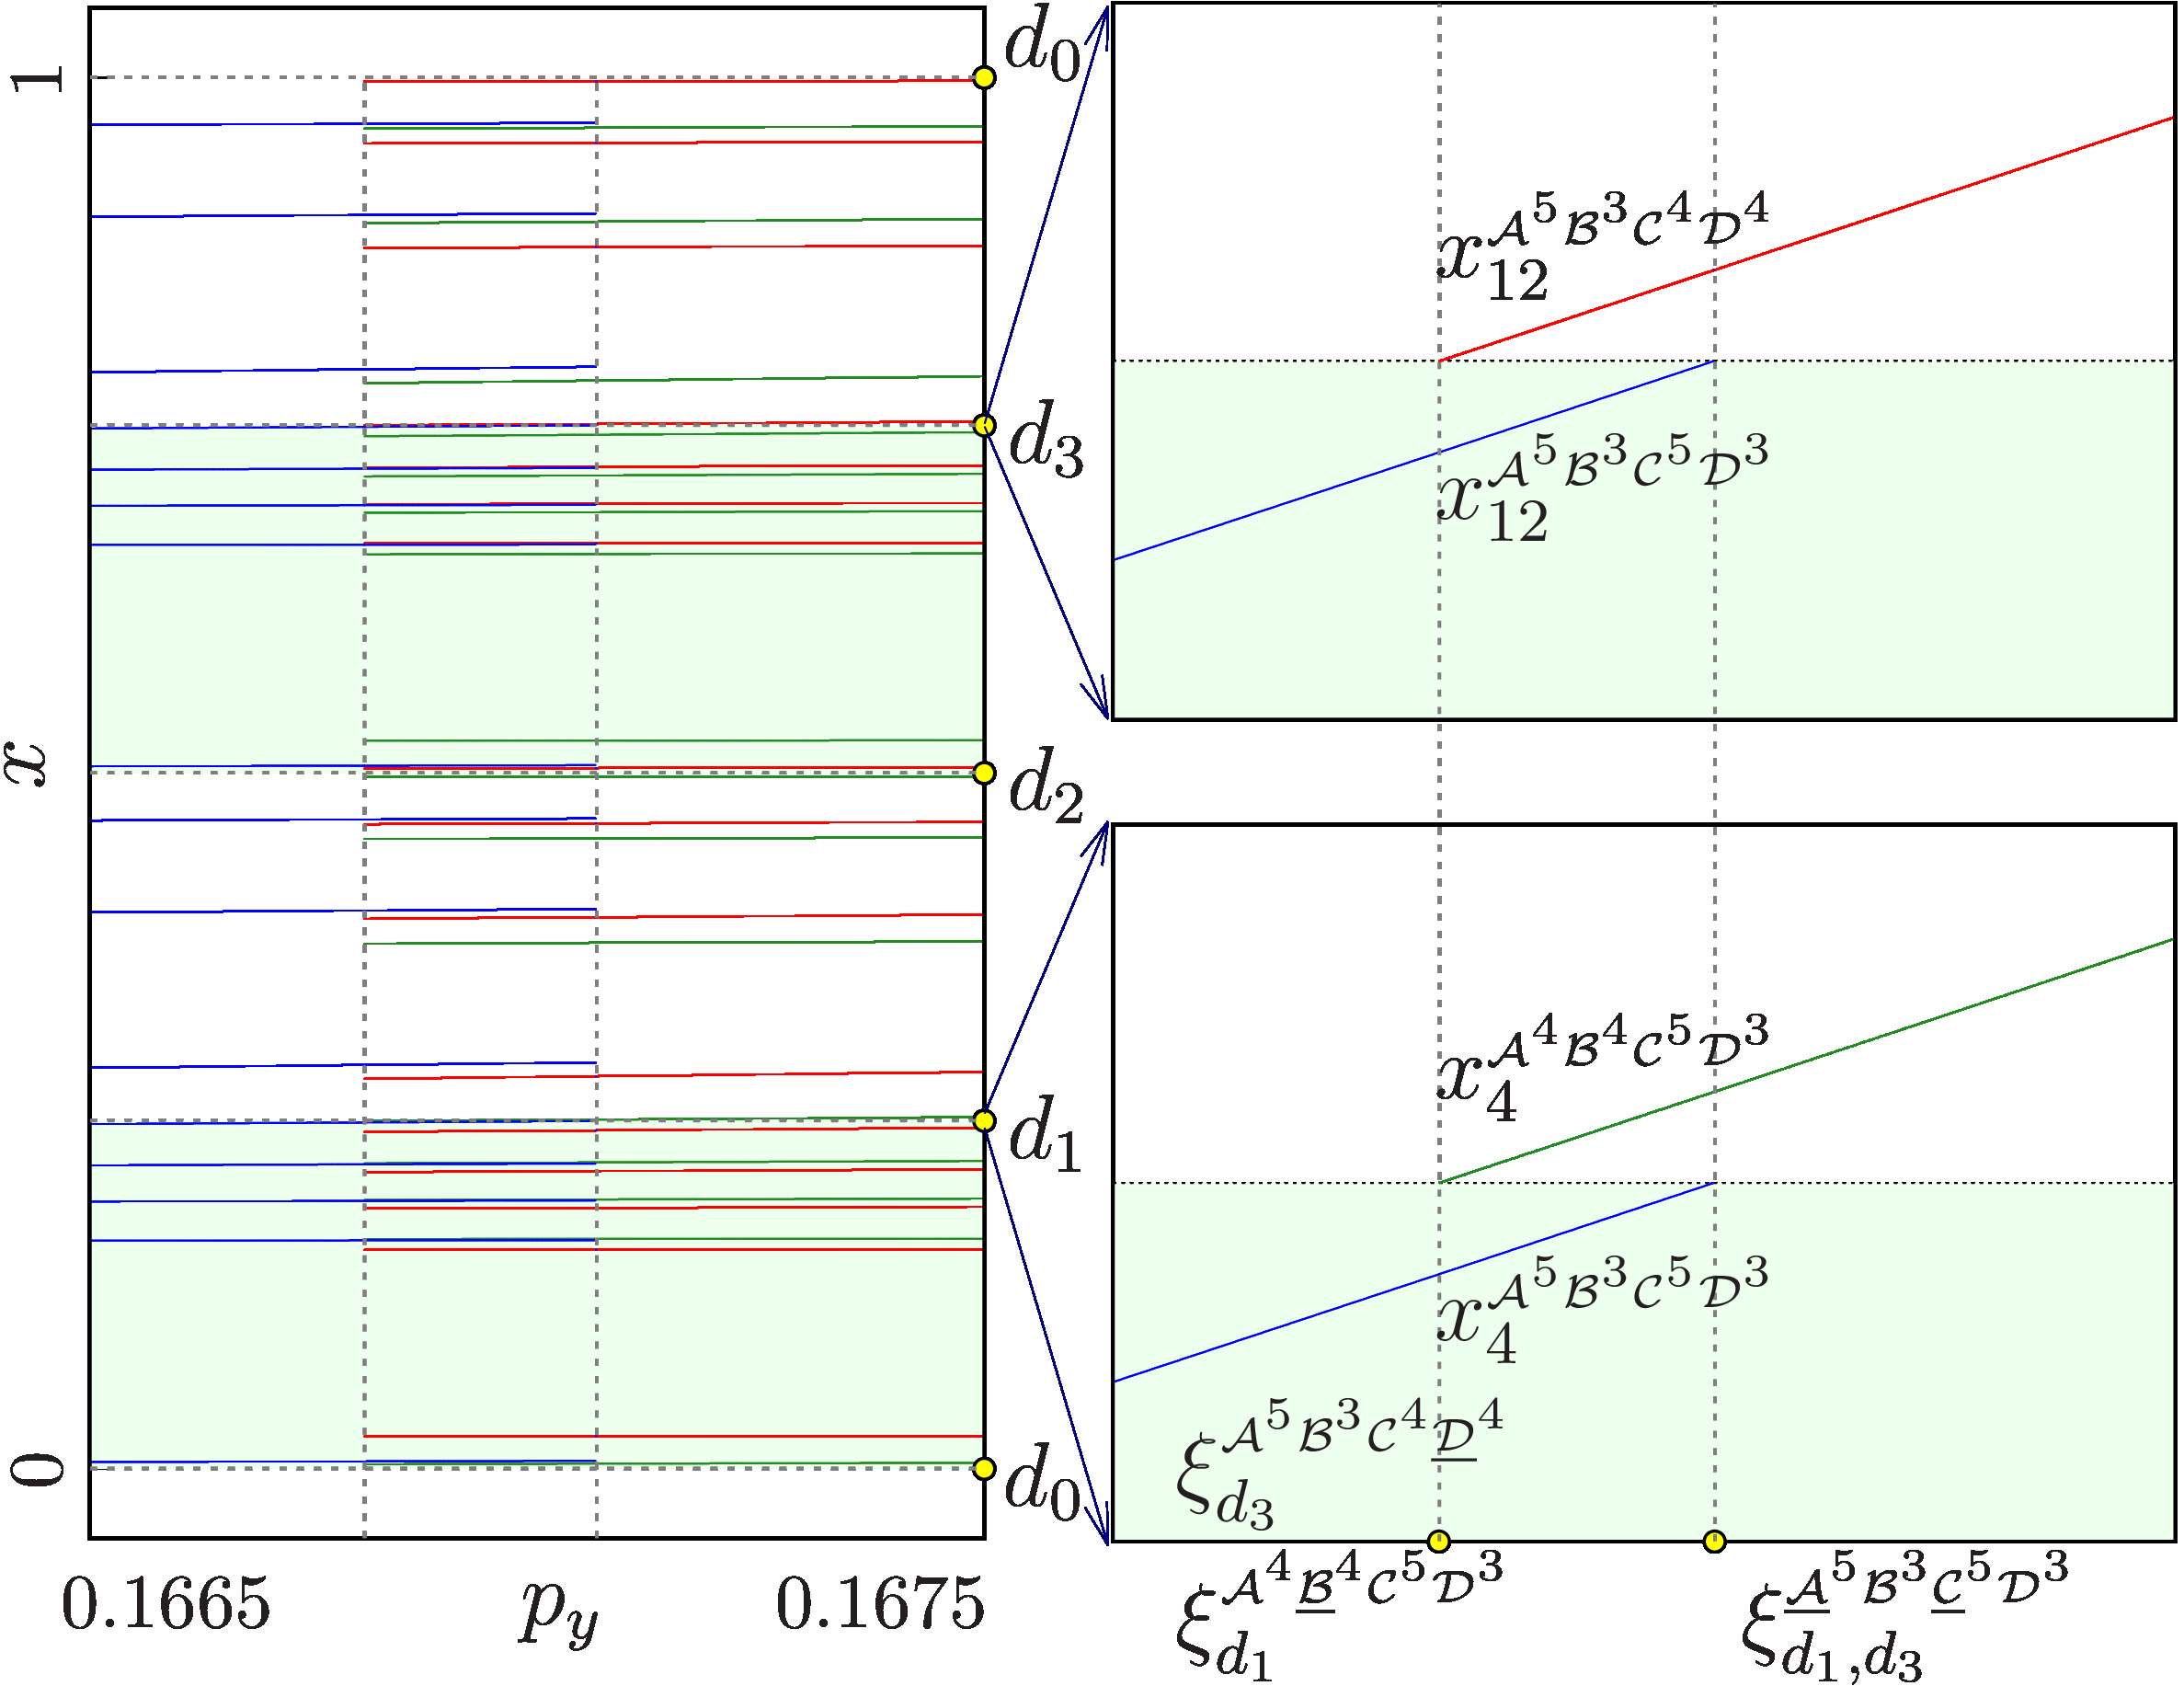
\includegraphics[height=.7 \textheight]{../Figures/6/6.5/result.png}}
					\caption*{$F_{16}^\downarrow$}
				}
				\only<4>{
					\subfloat{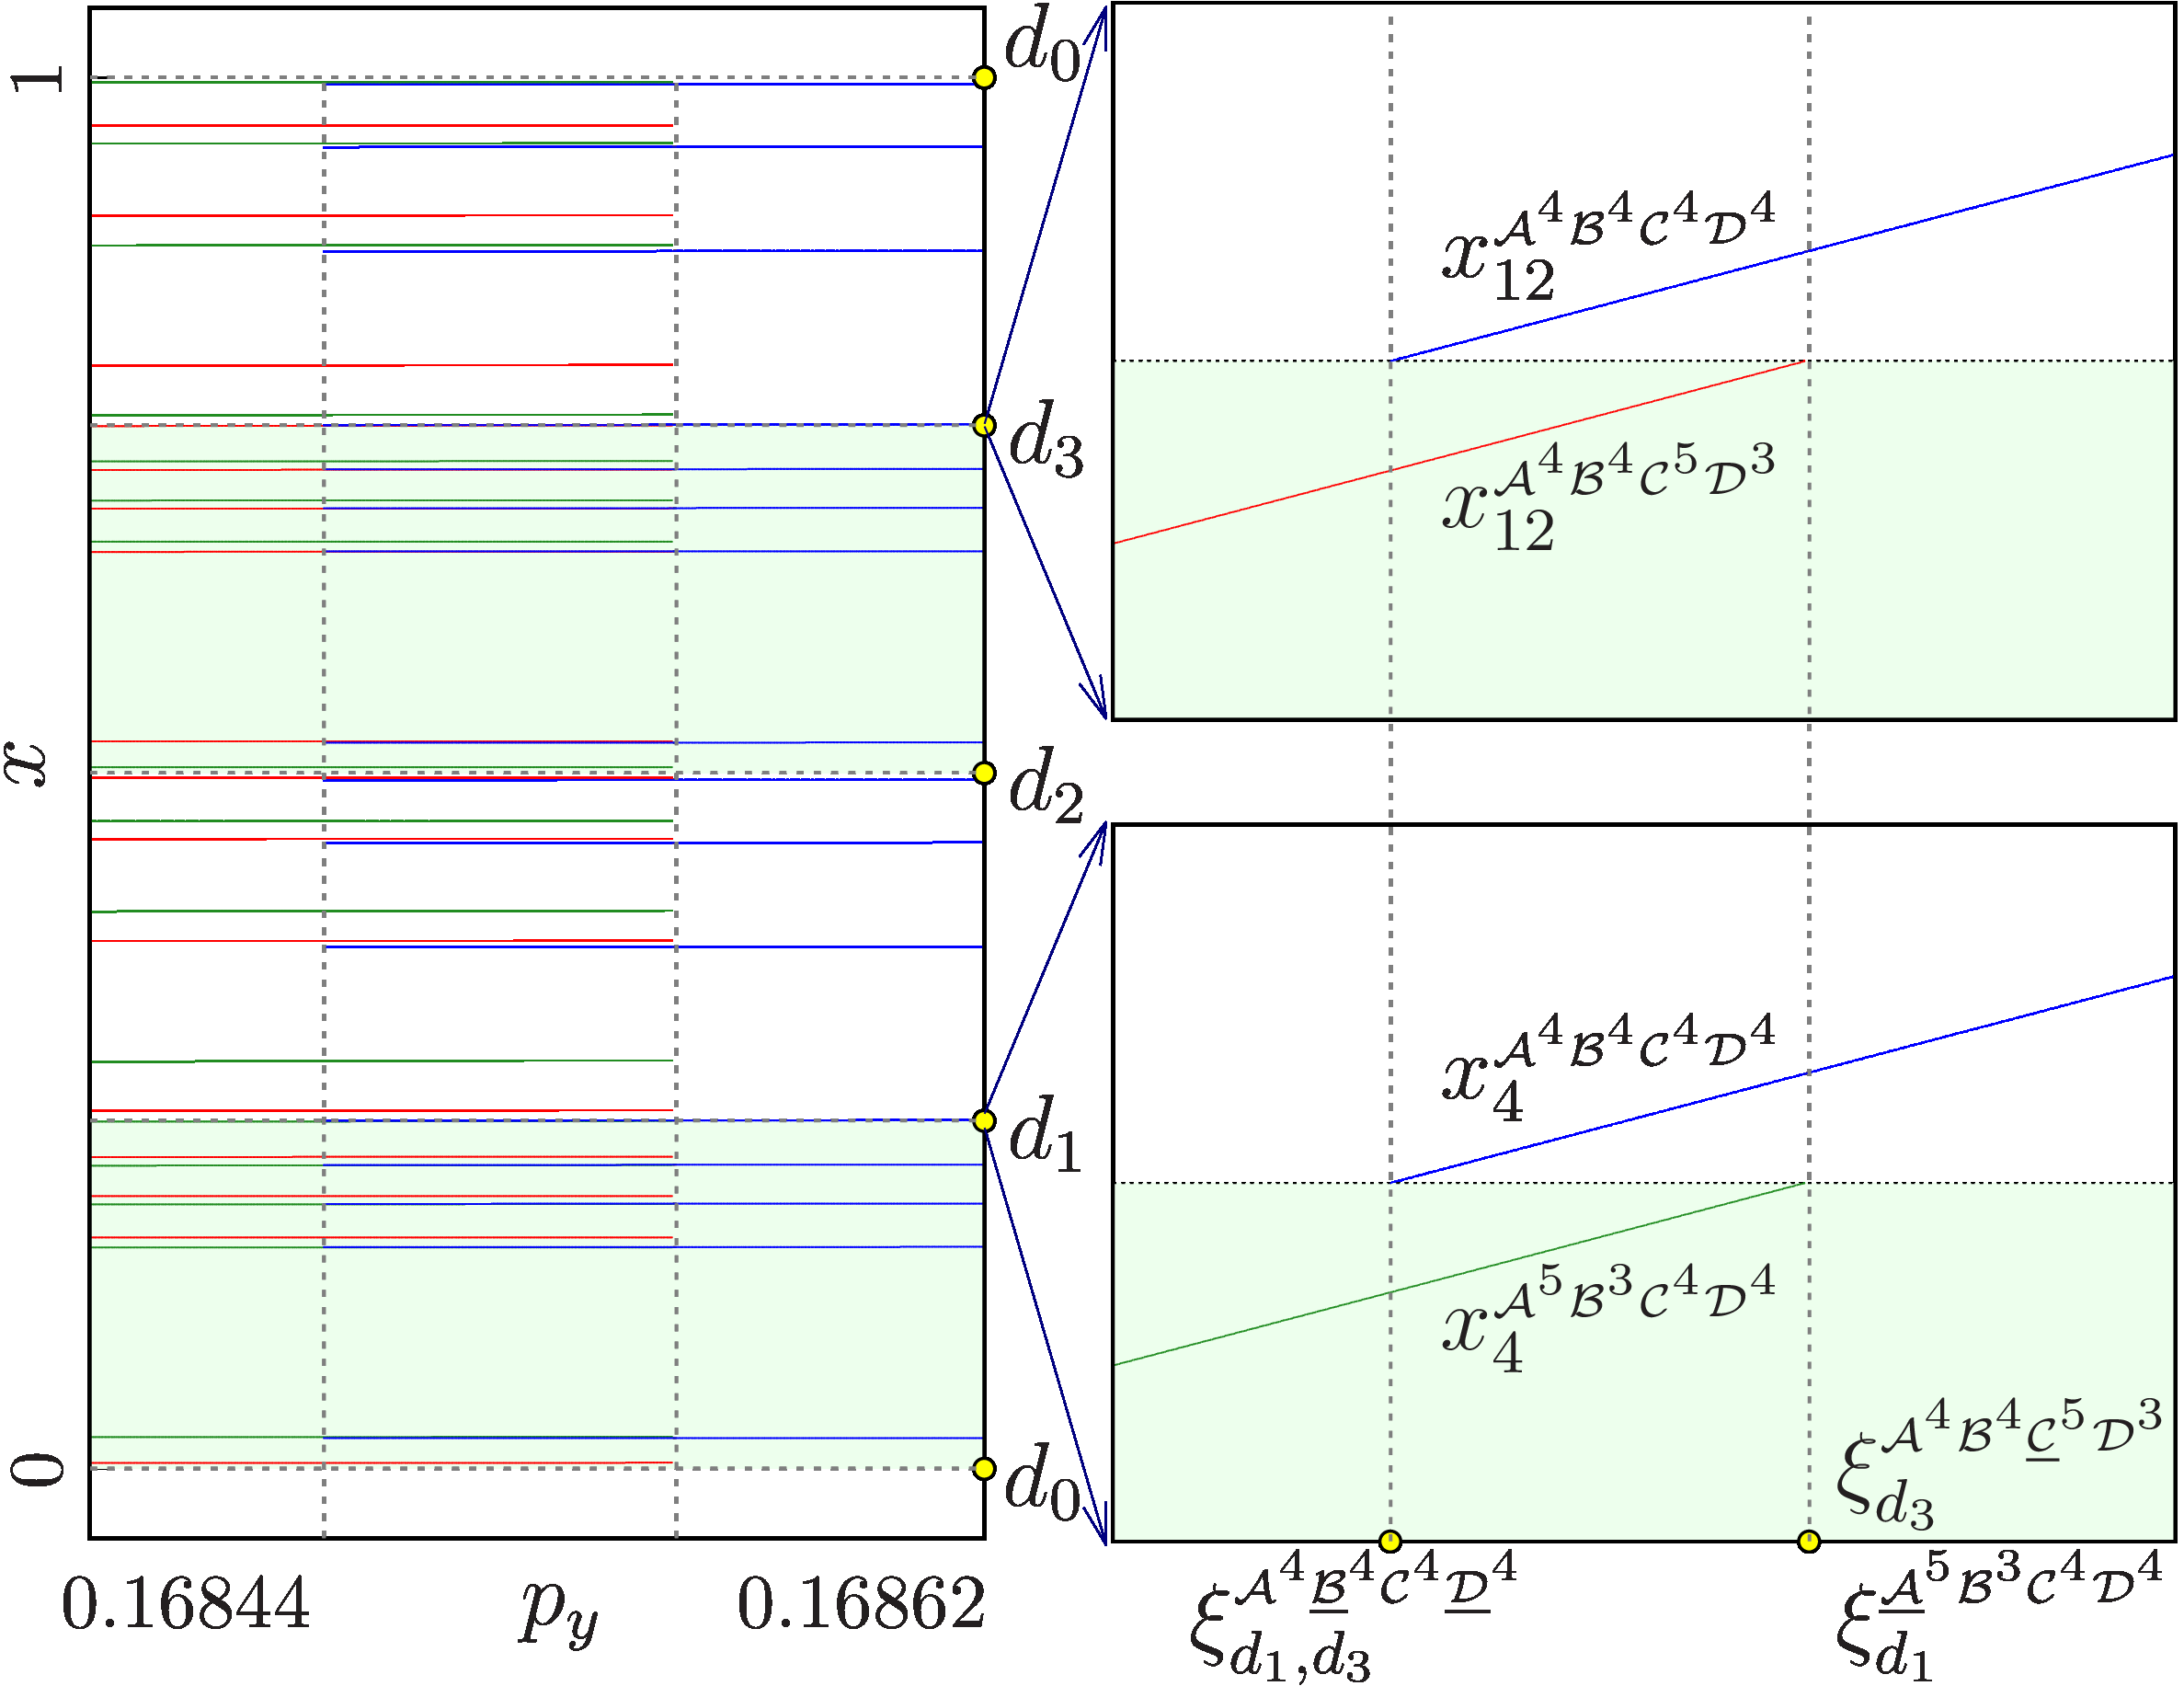
\includegraphics[height=.7 \textheight]{../Figures/6/6.6/result.png}}
					\caption*{$F_{16}^\leftarrow$}
				}
				\only<5>{
					\subfloat{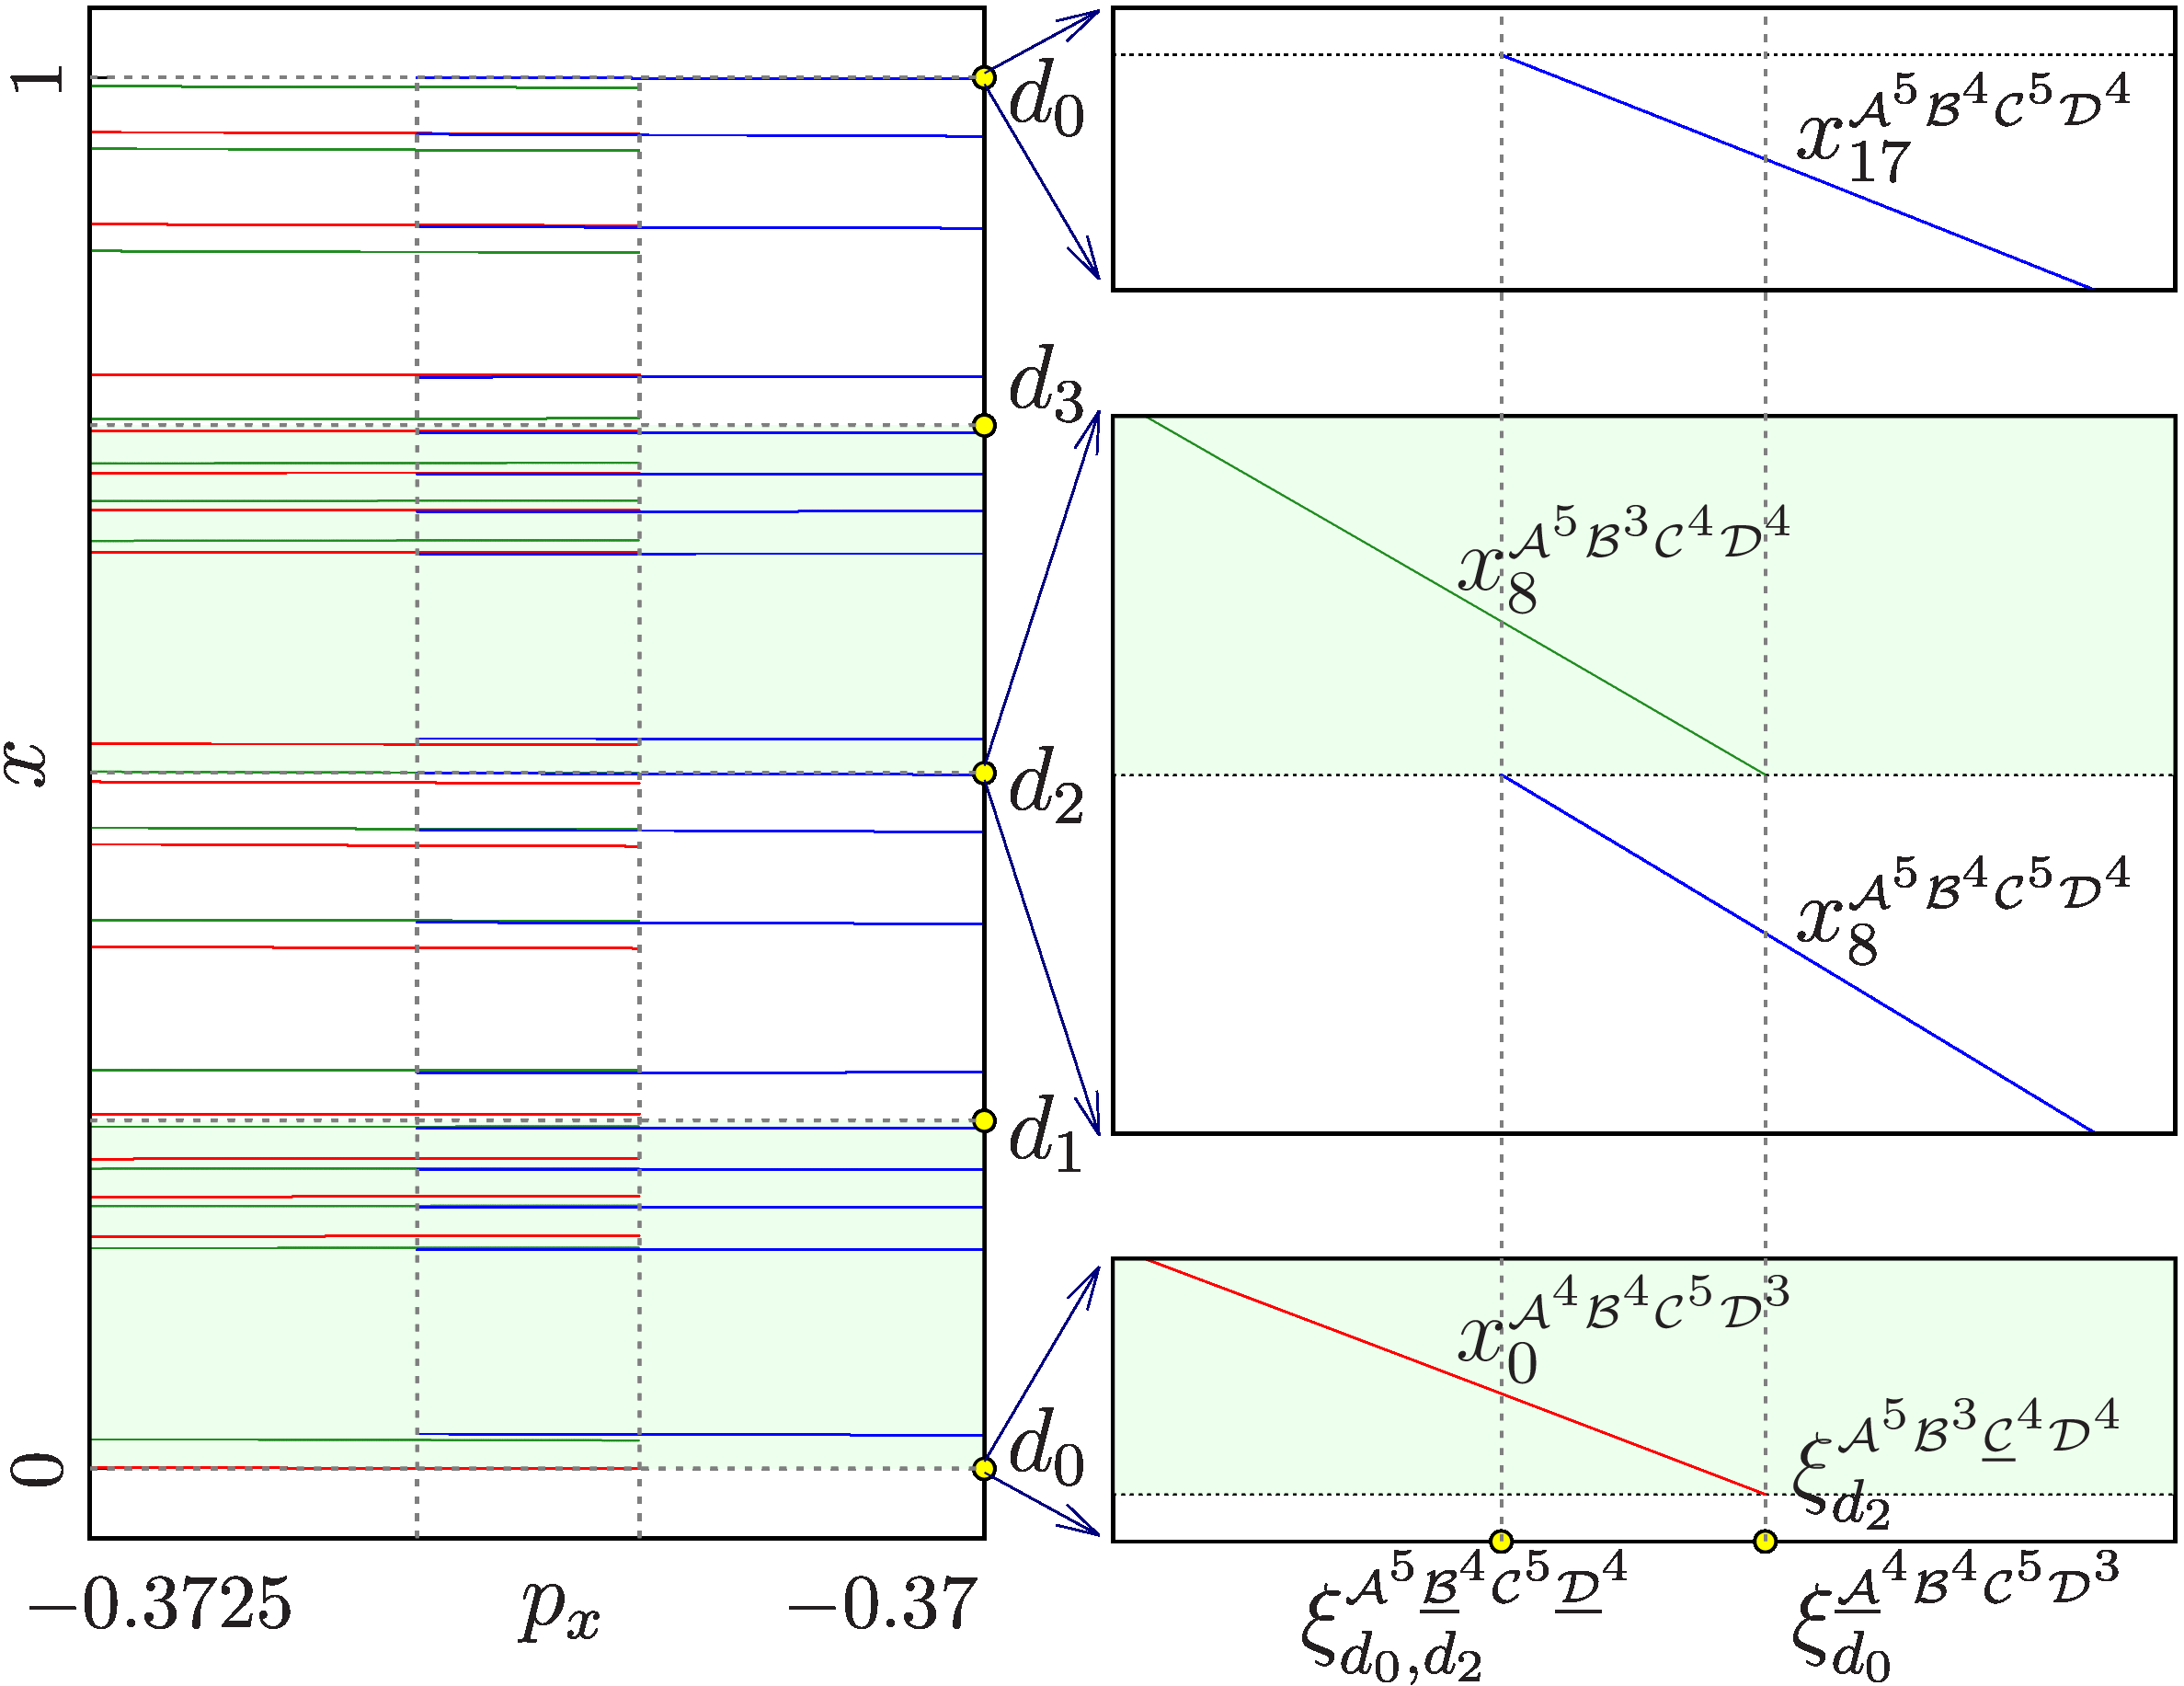
\includegraphics[height=.7 \textheight]{../Figures/6/6.7/result.png}}
					\caption*{$F_{16}^\rightarrow$}
				}
			\end{figure}
		\end{column}
	\end{columns}
\end{frame}

\begin{frame}{Bifurcation Regularities}
	\todo{List regularities}
\end{frame}

\begin{frame}{Overlapping Parameter Regions (1/2)}
	\todo{Scrap?}
	\vspace{-1em}
	\begin{columns}
		\begin{column}{.8 \textwidth}
			\vspace{-3em}
			\begin{figure}
				\centering
				\subfloat[``Type A'']{
					\includegraphics[height=0.7 \textheight]{60_MinimalRepr/2D_Regions_E/result.png}
				}
				\subfloat[``Type B'']{
					\includegraphics[height=0.7 \textheight]{60_MinimalRepr/2D_Regions_F/result.png}
				}
				\caption*{Overlapping period regions}
			\end{figure}
		\end{column}
		\begin{column}{.2 \textwidth}
			\vspace{-4em}
			\begin{figure}
				\subfloat{ \includegraphics[height=.3 \textheight]{60_MinimalRepr/2D_Regions_Whole/Manual/EF/result.png} }
			\end{figure}
		\end{column}
	\end{columns}
\end{frame}

\begin{frame}{Overlapping Period Regions (2/2)}
	\todo{Scrap?}
	\vspace{-1em}
	\begin{columns}
		\begin{column}{.5 \textwidth}
			Coexistence scenarios:
			\begin{itemize}
				\item<1-> 1: ``Type A'' ($L$)
				\item<1-> 2: Two different ``Type A'' \\ ($M, N, O,$ and $P$)
				\item<2-> 2: ``Type B'' pair ($Q$)
				\item<3-> 3: ``Type B'' pair and ``Type A'' \\ ($R, S, T,$ and $U$)
				\item<4-> 4: ``Type B'' pair \\ and two different ``Type A'' \\ ($V, W, X,$ and $Y$)
			\end{itemize}

			\vspace{.5em}
			\onslide<4->{
				The coexistence of 4 cycles was overlooked in the original model!
			}
		\end{column}
		\begin{column}{.5 \textwidth}
			\vspace{-5em}
			\begin{figure}
				\centering
				\subfloat{ \includegraphics[height=0.2 \textheight]{60_MinimalRepr/2D_Regions_E/result.png} }
				\subfloat{ \includegraphics[height=0.2 \textheight]{60_MinimalRepr/2D_Regions_F/result.png} }
				\only<1>{
					\subfloat{\includegraphics[height=.7 \textheight]{60_MinimalRepr/Cobweb_M/Manual/result.png}}
					\caption*{At point $M$}
				}
				\only<2>{
					\subfloat{\includegraphics[height=.7 \textheight]{60_MinimalRepr/Cobweb_Q/Manual/result.png}}
					\caption*{At point $Q$}
				}
				\only<3>{
					\subfloat{\includegraphics[height=.7 \textheight]{60_MinimalRepr/Cobweb_U/Manual/result.png}}
					\caption*{At point $U$}
				}
				\only<4>{
					\subfloat{\includegraphics[height=.7 \textheight]{60_MinimalRepr/Cobweb_X/Manual/result.png}}
					\caption*{At point $U$}
				}
			\end{figure}
		\end{column}
	\end{columns}
\end{frame}

%\begin{frame}{Summary of Results}
%	\begin{itemize}
%		\item Constructed a function with similar properties as the original function
%		\item Reproduced the bifurcation behavior of the original model
%		\item Investigated coexisting cycles (found something new!)
%		\item Investigated bifurcations
%	\end{itemize}
%
%	\pause
%	\vspace{2em}
%	This answers research questions 1 and 2
%\end{frame}

\begin{frame}{The Next Step}
	\todo{Reformulate results, next step in next part of the presentation}
	\vspace{-1em}
	Research questions:
	\begin{enumerate}
		\item Is there a simple model exhibiting the same behavior? \hfill \checkmark
		\item Was there something overlooked in the analysis of the original model? \hfill \checkmark
		      \pause
		\item What else can happen in the simplified model?
	\end{enumerate}

	\pause
	\vspace{1em}
	Hypothesis: Period Adding
	\begin{itemize}
		\item This is typical for models of power converters
		\item This is typical for piecewise increasing discontinuous models
		\item This is typical in between such chains of the same period
	\end{itemize}
\end{frame}
